\documentclass[times,10pt,twocolumn]{article}
\usepackage{ipdps}
\usepackage{vmargin}
\setpapersize{USletter}
\setmargnohf{0.8125in}{1in}{6.875in}{8.875in}
\pagestyle{empty}
\newenvironment{twoaffiliations}{\begin{tabular}{cc}}{\end{tabular}}
\newenvironment{oddaffiliation}{\begin{center}}{\\~\\\end{center}}
%\documentclass[times,11pt,onecolumn]{article} 
%\usepackage{latex8}
%\usepackage{times}
\usepackage{epsfig}
%\pagestyle{empty}
%\newcommand{\mt}[1]{\mbox{#1}}

\title{MPEG-2 Decoding in a Stream Programming Language}

\author{
  Matthew Drake, Hank Hoffmann, Rodric Rabbah, and Saman Amarasinghe\\
  \begin{twoaffiliations}
    Massachusetts Institute of Technology\\
    Computer Science and Artificial Intelligence Laboratory\\
    \{madrake, hank, rabbah, saman\}@mit.edu
  \end{twoaffiliations}
}

\begin{document}
  
  \maketitle
  \thispagestyle{empty}
  
  \begin{abstract}
    As DSP programming is becoming more complex, there is an increasing
need for high-level abstractions that can be efficiently compiled.
Toward this end, we present a set of aggressive optimizations that
target linear sections of a stream program.  Our input language is
StreamIt, which represents programs as a hierarchical graph of
autonomous filters.  A filter is linear if each of its outputs can be
represented as an affine combination of its inputs.  Linear filters
are common in DSP applications; examples include FIR filters,
expanders, compressors, FFTs and DCTs.

We present a linear extraction analysis that automatically detects
linear filters based on the C-like code in their {\tt work} function.
Once linear filters are identified, we show how neighboring nodes can
be collapsed into a single linear representation, thereby eliminating
many redundant computations.  Also, we describe a method for
automatically translating linear nodes into the frequency domain,
thereby yielding algorithmic savings for convolutional filters.

We have completed a fully-automatic implementation of the above
techniques as part of the StreamIt compiler, and we demonstrate
performance improvements that average 400\% over our benchmark
applications.




  \end{abstract}
  
  \section{Introduction}

Applications that are structured around some notion of a ``stream''
are becoming increasingly important and widespread.  There is evidence
that streaming media applications are already consuming most of the
cycles on consumer machines \cite{Rix98}, and their use is continuing
to grow.  In the embedded domain, applications for hand-held
computers, cell phones, and DSP's are centered around a stream of
voice or video data.  The stream abstraction is also fundamental to
high-performance applications such as intelligent software routers,
cell phone base stations, and HDTV editing consoles.

Despite the prevalence of these applications, there is surprisingly
little language and compiler support for practical, large-scale stream
programming.  Of course, the notion of a stream as a programming
abstraction has been around for decades \cite{SICP}, and a number of
special-purpose stream languages have been designed (see
\cite{survey97} for a review).  Many of these languages and
representations are elegant and theoretically sound, but they often
lack features and are too inflexible to support straightforward
development of modern stream applications, or their implementations
are too inefficient to use in practice.  Consequently, most
programmers turn to general-purpose languages such as C or C++ to
implement stream programs.

There are two reasons that general-purpose languages are inadequate for
stream programming.  Firstly, they are a mismatch for the application
domain.  That is, they do not provide a natural or intuitive
representation of streams, thereby having a negative effect on
readability, robustness, and programmer productivity.  Moreover, because
the widespread parallelism and regular communication patterns of data
streams are left implicit in general-purpose languages, compilers are
not stream-conscious and do not perform stream-specific optimizations.
As a result, performance-critical loops are often hand-coded in a
low-level assembly language and must be re-implemented for each target
architecture.  This practice is labor-intensive, error-prone, and very
costly.

Secondly, general-purpose languages are a mismatch for the emerging
class of grid-based architectures \cite{smartmemories,rawshort,trips} that
are especially well-suited for stream processing.  Perhaps the primary
appeal of C is that it provides a ``common machine language'' for
von-Neumann architectures.  That is, it abstracts away the
idiosyncratic differences between machines, but encapsulates their
common properties: a single program counter, arithmetic operations,
and a monolithic memory.  However, for grid-based architectures, the
von-Neumann model no longer holds, as there are multiple instruction
streams and distributed memory banks.  Thus, C no longer serves as a
common machine language--in fact, it provides the wrong abstraction
for the underlying hardware, and architecture-specific directives are
often needed to obtain reasonable performance.  Again, this greatly
complicates the job of the programmer and hampers portability.

StreamIt is a language and compiler specifically designed for modern
stream programming.  The StreamIt language has two goals: first, to
provide high-level stream abstractions that improve programmer
productivity and program robustness within the streaming domain, and
second, to serve as a common machine language for grid-based
processors.  At the same time, the StreamIt compiler aims to perform
stream-specific optimizations to achieve the performance of an expert
programmer.

This paper motivates, describes, and justifies the high-level language
features of StreamIt, version 1.0.  The major limitation of StreamIt
1.0 is that all flow rates in the streams must be static; applications
such as compression that have dynamically varying flow rates will be
the subject of future work.  A large set of applications can be
implemented with static rates, and while dynamic rates will require a
different runtime model, it will still be essential to fully analyse
and optimize static sub-sections in order to obtain high performance.

The paper is organized as follows. In Section {\ref{sec:domain}}, we
characterize the domain of streaming programs that motivates the
design of StreamIt, and in Section~\ref{sec:overview} we describe the
language features in detail.  We present an in-depth example of a
software radio in Section~\ref{sec:example}, preliminary results in
Section~\ref{sec:results}, related work in Section~\ref{sec:related},
and conclusions in Section~\ref{sec:conc}.


  \Section{MPEG-2 Video Coding and Decoding}

MPEG-2~\cite{MPEG2} is a popular coding and decoding standard
for digital video data. The scheme is a subset of both the
DVD-Video~\cite{Taylor:1999:SDV} standard for storing movies, and the Digital
Video Broadcasting specifications for transmitting HDTV and
SDTV~\cite{DVB}. The scheme is used by a wide variety of multimedia
applications and appliances such as the Tivo Digital Video
Recorder~\cite{tivo}, and the DirecTV satellite broadcast
service~\cite{directv}.

MPEG-2 encoding uses both {\it lossy} compression and {\it lossless}
compression. Lossy compression permanently eliminates information from
a video based on a human perception model. Humans are much better at
discerning changes in color intensity (luminance information) than
changes in color (chrominance information). Humans are also much more
sensitive to low frequency image components, such as a blue sky, than
to high frequency image components, such as a plaid shirt. Details
which humans are likely to miss can be thrown away without affecting
the perceived video quality.

Lossless compression eliminates redundant information while allowing
for its later reconstruction. Similarities between adjacent video
pictures are encoded using motion prediction, and all data is Huffman
compressed\cite{Huffman52}. The amount of lossy and lossless
compression depends on the video data. Common compression ratios range
from 10:1 to 100:1. For example, HDTV, with a resolution of 1280x720
pixels and a streaming rate of 59.94 frames per second, has an
uncompressed data rate of 1.33 Gigabits per second. It is compressed at
an average rate of 66:1, reducing the required streaming rate to
20 Megabits per second~\cite{imagevidstandards}. %% page 3: [p.3]

\SubSection{MPEG Coding}

%% \begin{figure}[t]
%% \begin{center}
%% \vspace{-12pt}
%% % \framebox{
%% % \includegraphics[scale=1, angle=0]{./mpeg-encoder.eps}
%% %}
%% % \vspace{-6pt}
%% % \nocaptionrule
%%  \caption{MPEG encoder.}
%%  \label{fig:mpeg-encoder}
%% %\vspace{-18pt}
%% \end{center}
%% \end{figure}

%% An overview of the encoding process is illustrated in
%% Figure~\ref{fig:mpeg-encoder}.
The encoder operates on a sequence of pictures. Each picture is made
up of a 16x16 grouping of pixels known as a macroblock.  A macroblock
consists of a 2x2 array of blocks, each of which contains an 8x8 array
of subpixels (i.e., individual color components of a pixel).
Macroblocks specify colors using a luminance channel to represent
saturation (color intensity), and two chrominance channels to
represent hue. Becuae the human eye is more sensitive to changes in
saturation than changes in hue, the chrominance channels are
frequently downsampled. The type of downsampling an MPEG-2 encoder
uses is known as the chrominance (chroma) format. The most common
chroma format is 4:2:0, which uses one 8x8 block for each of the
chrominance channels, downsampling a macroblock from 16x16 to 8x8
subpixels. An alternate format is 4:2:2. It uses two blocks for each
chrominance channel, downsampling each of the channels from 16x16 to
8x16 subpixels. The two chrominance formats are shown in
Figure~\ref{fig:chroma}.

The compression in MPEG is achieved largely via motion estimation,
which detects and eliminates similarities between macroblocks across
pictures. Specifically, the motion estimator calculates a motion
vector that represents the horizontal and vertical displacement of a
given macroblock (i.e., the one being encoded) from a matching
macroblock-sized area in a reference picture.  The matching macroblock
is removed (subtracted) from the current picture on a pixel by pixel
basis, and a motion vector is associated with the macroblock
describing its displacement relative to the reference picture. The
result is a residual predictive-code (P) picture. It represents the
difference between the current picture and the reference
picture. Reference pictures encoded without the use of motion
prediction are intra-coded (I) pictures. In addition to forward motion
prediction, it is possible to encode new pictures using motion
estimation from both previous and subsequent pictures. Such pictures
are bidirectionally predictive-coded (B) pictures, and they exploit a
greater amount of temporal locality.

Each of the I, P, and B pictures then undergoes a 2-dimensional
discrete cosine transform (DCT) which separates the picture into parts
with varying visual importance. The input to the DCT is one block.
The output of the
DCT is an 8x8 matrix of frequency coefficients. The upper left corner
of the matrix represents low frequencies, whereas the lower right
corner represents higher frequencies. The latter are often small and
can be neglected without sacrificing human visual perception.

%\begin{figure}[t]
%\begin{center}
%\vspace{-12pt}
%\framebox{
% \includegraphics[scale=.5, angle=0]{./zigzag.eps}
%}
% \vspace{-6pt}
 %\nocaptionrule
% \caption{Zig-Zag scan patterns. (a) shows the default scan pattern, while (b) shows the alternate scan pattern.}
% \label{fig:zigzag}
%\vspace{-18pt}
%\end{center}
%\end{figure}

The DCT coefficients are quantized to reduce the number of bits needed
to represent them. Following quantization, many coefficients are
effectively reduced to zero. The DCT matrix is then run-length encoded
by emitting each non-zero coefficient,
% TODO: clarify ``followed by the number of zeros that precede it''?
followed by the number of zeros that precede it, along with the number
of bits needed to represent the coefficient, and its value. The
run-length encoder scans the DCT matrix in a zig-zag order
(Figure~\ref{fig:zigzag-order}) to consolidate the zeros in the matrix.

Finally, the output of the run-length encoder, motion vector data,
and other information (e.g., type of picture), are Huffman coded to
further reduce the average number of bits per data item. The compressed
stream is sent to the output device.

\SubSection{MPEG Decoding}

An MPEG-2 decoder input stream is organized as a Group of Pictures
(GOP) which contains all the information needed to reconstruct a
video. The GOP contains the three kinds of pictures produced by the
encoder, namely I, P, and B pictures. I pictures are intended to
assist scene cuts, random access, fast forward, or fast reverse
playback~\cite[p. 14]{MPEG2}. A typical I:P:B picture ratio in a GOP
is 1:3:8, and a typical picture pattern is a repetition of the
following logical sequence:
I$_1$~B$_2$~B$_3$~P$_4$~B$_5$~B$_6$~P$_7$~B$_8$~B$_9$~P$_{10}$~B$_{11}$~B$_{12}$
where the subscripts denote positions in the original video.  However,
to simplify the decoder, the encoder reorders the pictures to produce
the following pattern:
I$_1$~P$_4$~B$_2$~B$_3$~P$_7$~B$_5$~B$_6$~P$_{10}$~B$_8$~B$_9$~B$_{11}$~B$_{12}$.
Under this configuration, if the decoder encounters a P picture, its
motion prediction is with respect to the previously decoded I or P
picture; if the decoder encounters a B picture, its motion prediction
is with respect to the previously two decoded I or P pictures.

As with the encoding process, pictures are divided up into 16x16 pixel
macroblocks composed of 8x8 blocks. There is a separate series of
macroblocks for the luminance and chrominance color channels.
%% \begin{figure}[t]
%% \begin{center}
%% \vspace{-12pt}
%% % \framebox{
%% % \includegraphics[scale=1, angle=0]{./mpeg-decoder.eps}
%% %}
%% % \vspace{-6pt}
%% % \nocaptionrule
%%  \caption{MPEG decoder.}
%%  \label{fig:mpeg-decoder}
%% %\vspace{-18pt}
%% \end{center}
%% \end{figure}
%% is illustrated in Figure~\ref{fig:mpeg-decoder}. It
The decoding process is conceptually the reverse of the encoding
process. The input stream is Huffman and run-length decoded, resulting
in quantized DCT matrices. The DCT coefficients are scaled in
magnitude and an inverse DCT (IDCT) is performed.
%% maps the frequency matrices to the spatial domain.
Finally, the motion vectors parsed from the data stream are passed to
a motion compensator, which reconstructs the original pictures. 
%% In the
%% case of I pictures, the compensator need not make any changes since
%% these pictures were not subject to motion estimation\footnote{I
%% pictures may contain concealment motion vectors which aid in
%% macroblock reconstruction should a bitstream error destroy the
%% frequency coefficient data. We ignore this special case.}. In the case
%% of P and B pictures however, motion vectors are used to find the
%% corresponding region in the current reference pictures. The
%% compensator then adds the relevant reference macroblocks to the
%% current picture to reconstruct it. These pictures are then emitted to
%% an output device.
  \section{StreamIt}
\label{sec:streamit}

StreamIt  is   an  architecture independent language that is
designed for  stream programming. In StreamIt, programs are
represented as graphs where  nodes represent  computation and edges
represent FIFO-ordered communication of data over tapes.

\paragraph*{Hierarchical Streams}
In  StreamIt, the  basic programmable  unit (i.e., an actor) is a {\it
filter}.   Each filter contains  a work  function that executes
atomically,  popping (i.e., reading)  a fixed number  of items  from
the  filter's input  tape and pushing (i.e., writing) a fixed number
of items to the filter's output tape.  A filter  may also {\tt peek} at
a given index  on its input tape without  consuming  the  item;  this
makes  it  simple  to  represent computation over a
sliding window.   The {\tt push}, {\tt pop}, and {\tt peek} rates are
declared as part  of  the work  function,  thereby enabling  the
compiler    to construct a static schedule of filter executions. The
following is an example implementation of a Finite Impulse
Response (FIR)  filter: 

\begin{scriptsize}
% {\small
\begin{verbatim}
float->float filter FIR (int N, float[] weights) 
{
  work push 1 pop 1 peek N {
    float sum = 0;
    for (int i = 0; i < N; i++) {
      sum += peek(i) * weights[i];
    }
    pop();
    push(sum);
  }
}
\end{verbatim}
% }
\end{scriptsize}

The work function is invoked (fired) whenever there is sufficient data
on the input tape. For the FIR example above, the filter requires at least
\texttt{N} elements before it can execute. The value of \texttt{N} is
known at compile time when the filter is composed to form a stream
graph. A filter is akin to a class in object oriented programming
with the work function serving as the main method. The parameters
to a filter (e.g., \texttt{N} and \texttt{weights}) are equivalent to
parameters passed to a class constructor. 

\begin{figure}[t]
\begin{center}
%\vspace{-24pt}
% \framebox{
 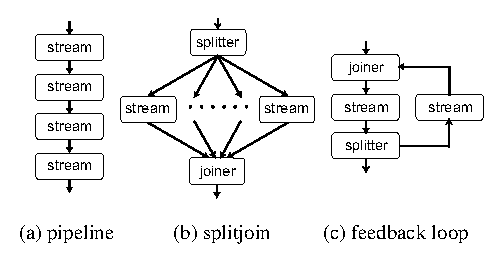
\includegraphics[scale=1, angle=0]{./constructs-eg.eps}
%}
% \vspace{-6pt}
% \nocaptionrule
 \caption{Hierarchical streams in StreamIt.}
 \label{fig:containers}
\end{center}
\end{figure}

\begin{figure}[t]
\begin{center}
\vspace{-12pt}
% \framebox{
 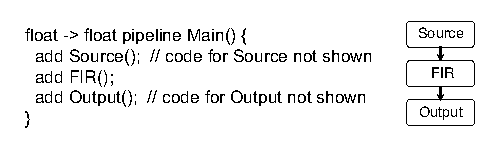
\includegraphics[scale=1, angle=0]{./pipeline-eg.eps}
%}
% \vspace{-6pt}
% \nocaptionrule
 \caption{Example pipeline with FIR filter.}
 \label{fig:pipeline}
%\vspace{-18pt}
\end{center}
\end{figure}

In StreamIt, the
application developer focuses on the hierarchical assembly of the
stream graph and its communication topology, rather than on the 
explicit management of the data buffers between filters.
StreamIt provides three hierarchical structures for composing filters
into larger stream graphs (see Figure~\ref{fig:containers}). The 
{\it pipeline} construct composes streams in sequence, with the output
of one connected to the input of the next.   An example of a pipeline
appears in Figure~\ref{fig:pipeline}.

The {\it splitjoin} construct distributes data to a set of parallel
streams, which are then joined together in a round robin fashion.  In
a splitjoin, the {\it splitter} performs the data scattering, and the
{\it joiner} performs the gathering. A splitter is a specialized
filter with a single input and  multiple output channels. On 
every execution step, it can distribute its output to any one of
its children in either a {\it duplicate} or a {\it roundrobin}
manner. For the former, incoming data are replicated to every
sibling connected to the splitter. For the latter, data are scattered
in a round robin manner, with each item sent to exactly one child
stream, in order.  The splitter type and the weights for distributing data to
child streams are declared as part of the syntax (e.g., \texttt{split
duplicate} or \texttt{split roundrobin($w_1,\ldots,w_n$)}). The
splitter counterpart is the joiner. It is a specialized filter with  
multiple input channels but only one output channel. The joiner
gathers data from its predecessors in a round robin manner (declared
as part of the syntax) to produce a single output stream.

StreamIt also provides a {\it feedback loop} construct for introducing
cycles in the graph.

%\section{Execution Model}
%\label{sec:execmodel}

%% A StreamIt program is represented by a hierarchical graph,
%% where the leaf nodes are filters, splitters, and joiners, and
%% the composite nodes are pipelines, splitjoins, and
%% feedback-loops. Edges in the graph represent data channels, which 
%% operate as FIFO queues.
\paragraph*{Execution Model}
As noted earlier, an actor (i.e., a filter, splitter, or joiner)
executes whenever there are enough data items on its input 
tape. In StreamIt, actors have  two epochs
of execution: one for initialization, and one for the {\it steady
state}. The initialization primes the input tapes to allow filters with
peeking to execute the very first instance of their work functions.
%%initialization in this setting is similar to the prologue stage in
%%software pipelining. 
A steady state is an execution that does not change the
buffering in the channels: the number of items on each channel
after the execution is the same as it was before the execution. 
Every valid stream graph has a steady state~\cite{LM87-i}, and within
a steady state, there are often many possibilities for interleaving
actor executions. 
%% The steady state schedule has the property that
%% the amount of data buffered between any two actors does not change
%% before and after the actor executions.
\begin{figure}[t]
\begin{center}
%%\vspace{-24pt}
%\vspace{24pt}
 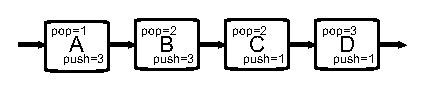
\includegraphics[scale=1, angle=0]{./pipe-with-rates.eps}
%\vspace{-6pt}
% \nocaptionrule
 \caption{Example pipeline.}
 \label{fig:pipe-with-rates}
\end{center}
%\vspace{-12pt}
\end{figure}
An example of a steady state for the pipeline in
Figure~\ref{fig:pipe-with-rates} requires filter \texttt{A} to fire
4 times, \texttt{B} 6 times, \texttt{C} 9 times, and
\texttt{D} 3 times. 
% Because in StreamIt the filters are
% independent (i.e., they do not share state), they can execute
% concurently. In a uniprocessor setting (which is what we use for our
% evaluation), we can only run one filter at time. Therefore, 
% The data generated by one actor are buffered (cached) until they are
% consumed.

\paragraph*{Compilation Process}
The StreamIt compiler derives the initialization and steady state
schedules~\cite{karczma-lctes03} and outputs a C program that includes
the initialization and work functions, as well as a driver to execute
each of the two schedules. Our compilation process allows the StreamIt
compiler to focus on high level optimizations, and relies on existing
compilers to perform machine-specific optimizations such as register
allocation, instruction scheduling, and 
code generation---this two step approach affords us a
great deal of portability (e.g., code generated from the StreamIt
compiler is compiled and run on three different machines as reported
in Section~\ref{sec:evaluation}).

%% For example, referring to
%% Figure~\ref{fig:pipe-with-rates}, the compiler generates the following
%% sample code for running the steady state schedule:
%% %\begin{scriptsize}
%% \begin{verbatim}
%% run_steady_state() {
%%   for (i = 0; i < 4; i++) A_work();
%%   for (i = 0; i < 6; i++) B_work();
%%   for (i = 0; i < 9; i++) C_work();
%%   for (i = 0; i < 3; i++) D_work();
%% }
%% \end{verbatim}
%% %\end{scriptsize}
%% To execute the program, the steady state is wrapped with
%% another loop that invokes the steady state a designated number of
%% times. Preceding the state steady, a similar initialization schedule
%% is run to prime the data buffers.
%, and following the steady state, an
%epilogue is run to drain the buffers as necessary.

%% \begin{figure}[t]
%% \begin{center}
%% \vspace{-12pt}
%%  \psfig{figure=ssi.eps,width=3in}
%%  \vspace{-6pt}
%%  \caption{Instruction size (in bytes along the y-axis) per filter
%%  (x-axis) occurring in a steady state execution of FFT.}
%%  \label{fig:ssi-single}
%% \vspace{-18pt}
%% \end{center}
%% \end{figure}

  \Section{MPEG Decoder in StreamIt}

The MPEG decoder pipeline is shown in
Figure~\ref{fig:dec-with-code}. The stream graph is shown on the
left. The StreamIt code is shown on the right, and it is correlated
with the stream block level diagram.

%% The decoder accepts a compressed bit stream as input, and produces the
%% decoded video stream as output.
The computation is encapsulated in three main components:
the parser (line 8), the block and motion vector decoder (lines 9-22),
and the motion compensator (lines 23-32).
The parser is responsible for parsing the MPEG-2 bit stream and
performing Huffman and variable run-length decoding (VLD). The output
of the VLD is an interleaved stream of quantized macroblocks encoded
in the frequency-domain, and offset-encoded motion vectors. The VLD
outputs $\texttt{N}\times\texttt{B}$ data elements for each
macroblock, followed by \texttt{V} data elements that encode its
motion vector. The actual value of \texttt{N} depends on the chroma
format. In a 4:2:0 chroma format regime, $\texttt{N}=6$ since each
macroblock consists of four 8x8 subpixel blocks for the luminance
channel, and two 8x8 subpixel blocks for the two chrominance
channels. Therefore, the VLD outputs a total of six 8x8 blocks, or 384
subpixels per macroblock. However, the total number of macroblocks
that are output by the parser is dependent on the number of frames in
the input encoded video. As a result, the VLD has a variable I/O
rate. The VLD filter is the only variable rate filter in the decoder
pipeline.

The VLD output is segregated into two homogeneous streams by a
roundrobin splitter (line 10). The first stream undergoes inverse
transformations (lines 11-16), while the second is decoded to produce
absolute motion vectors (lines 17-20). As is evident from the computation
graph, the two streams are decoded in parallel, and then merged (line
21) prior to the motion compensation stage of the pipeline.

The inverse transformations map each 8x8 block from the frequency
domain back to the spatial domain. Each block is reordered
(line 12), and then inversely quantized (line 13). This is followed by
an inverse DCT and a bounded saturation filter (lines 14-15). The set
of transformations is grouped into a pipeline whose input
and output types are automatically inferred by the compiler. Each of
the filters in this pipeline operate on 8x8 blocks. The code that is
shown does not take advantage of data level parallelism between
blocks. It is rather straightforward however to expose this
parallelism if it is desirable. For example, in this case a splitjoin
can replicate the inverse transformation pipeline $N$ times:
\begin{center}
  \begin{scriptsize}
    \begin{verbatim}
      add splitjoin {
        split roundrobin(B);
        for (int i = 0; i < N; i++) 
        // add pipeline
        join roundrobin(B);
      }
    \end{verbatim}
  \end{scriptsize}
\end{center}
\vspace{-12pt}
A stream-aware compiler can also automatically adjust the execution
granularity as necessary~\cite{gordon02asplos}, since data-parallel streams
can be easily identified as those that are stateless (i.e., do not
carry mutable state from one iteration to the next).

The third stage of the decoding pipeline performs the motion
compensation (lines 23-32) to recover predictively coded
macroblocks. The motion compensation filter uses the motion vectors to
find a corresponding macroblock in a previously decoded reference
picture. The reference macroblock is added to the current macroblock
to recover the original picture data. If the current macroblock is
part of an I or P picture, then the decoder stores it for use as a
future reference picture.

In the compensation stage, there are three parallel streams.  The
first handles the luminance color channel (Y), and the other two
handle the chrominance channels (Cb and Cr). The roundrobin splitter
(line 24) distributes the macroblocks according to the chroma
format. Since the luminance channel is not downsampled during the
encoding process, the splitter dispatches four 8x8 blocks at a time to
the Y motion compensator. The chrominance channels are typically
downsampled by a factor of 4, and hence one 8x8 block is streamed to
each of the Cb and Cr pipelines, which upsample (line 29) the results
of the motion compensator to generate the full 16x16 macroblock.  The
upsampling is a linear interpolation of the surrounding pixels.
The joiner (line 31) assembles the pictures from each of the color
channels, one pixel at a time.  The output is then readied for display
(lines 33 and 34) by organizing the pictures in accord with their
temporal order, and performing color space conversion to the RGB (red,
green, blue) color model. Note that these two filters each consume
$3\times\texttt{W}\times\texttt{H}$ subpixels per picture. This is
three times the pixel resolution of the decoded image since there is
one pixel generated from each of the three channel decoders. The final
output of the decoder is $\texttt{W}\times\texttt{H}$ pixels.  In
contrast to the filters for motion compensation and inverse transformation,
whose I/O rates are statically resolved at compile time, the picture 
reordering and color space conversion have I/O rates that are
parameterized on initialization time constants, namely the pixel
resolution of the pictures.

%% The MPEG-2 decoder in StreamIt is a fully portable implementation in
%% that the application is not architecture dependent. The implementation
%% naturally exposes the pipeline parallelism that exists throughout the
%% decoder, as well as the data level parallelism inherent to the inverse
%% transformations and motion compensation.  

The decoder implementation was carried out by one student programmer
with no prior understanding of MPEG. The development spanned eight
weeks from specification~\cite{MPEG2} to the first fully functional
MPEG decoder. The StreamIt code is nearly 3,165 lines of code with 48
static streams. The bit stream parser is the largest single filter,
consisting of 775 lines of code. The 48 static streams compile to
2,150 instantiated filters\footnote{A  {\it static stream} is a unique
code block, which may have multiple instantiations. For instance,
\texttt{MotionCompensation()} is a single filter with three
instantiations.} at a picture resolution of 352x240. By way of
comparison, the reference C implementation~\cite{reference-mpeg-c} is
6,835 lines of code\footnote{Line counts were generated using  the
\texttt{SLOCcount} tool. It strips whitespace and comments.}.  A line
count comparison is not an accurate measure of programmability, since
our StreamIt decoder implements only a subset of several stream types
supported by MPEG.  Our decoder does provide full support for the
range of different compression techniques used within MPEG, but
supports only a subset of the possible display modes (i.e. interlaced
versus progressive output).  However, these alternate display formats
represent minor conceptual changes and should therefore affect small
portions of the StreamIt code. This is demonstrated in
Section~\ref{section:chroma} with an example that illustrates how to
support multiple chrominance formats.

The reference C implementation intermingles parsing, decoding, and
motion compensation, making it difficult to clearly follow the code,
and hindering a better comparison. The C code also relies on global
variables to communicate values, such as quantization coefficients,
from the parser to the relevant code regions. In StreamIt, such
communication is relegated to teleport messaging (lines 13, 25, 28, and
33, and illustrated with dotted lines in
Figure~\ref{fig:dec-with-code}). For instance, the parser (VLD)
generates a message whenever the picture or macroblock type
changes. The motion compensation filters receive this information via
their dedicated portal (line 28), determine how to process the current
picture, and decide whether they needs to store the picture for future
reference. Note however that while there are multiple motion compensators
subscribed to the same portal, they each receive the same message with
respect to their local execution.
The picture reordering filter receives a similar message
(via portal on line 33), and uses the information to determine the
correct temporal order of pictures. The inverse transformation
pipeline listens to its portal (line 13) to determine the algebraic
manipulation required to perform the inverse quantization of the input
macroblock. Teleport messaging 
%% proves as a natural mechanism because
%% the macroblock type and picture type information changes infrequently
%% and irregularly, compared to the regular flow of data in the
%% application. Moreover, by 
exposes the flow of messages to the compiler, and allows for large
scale reordering or parallelization of the application without a
heroic dependence analysis. It also provides a mechanism to easily
introduce dynamic behavior into an otherwise static processing pipeline.

%% \begin{figure*}[b]
%%   \centerline{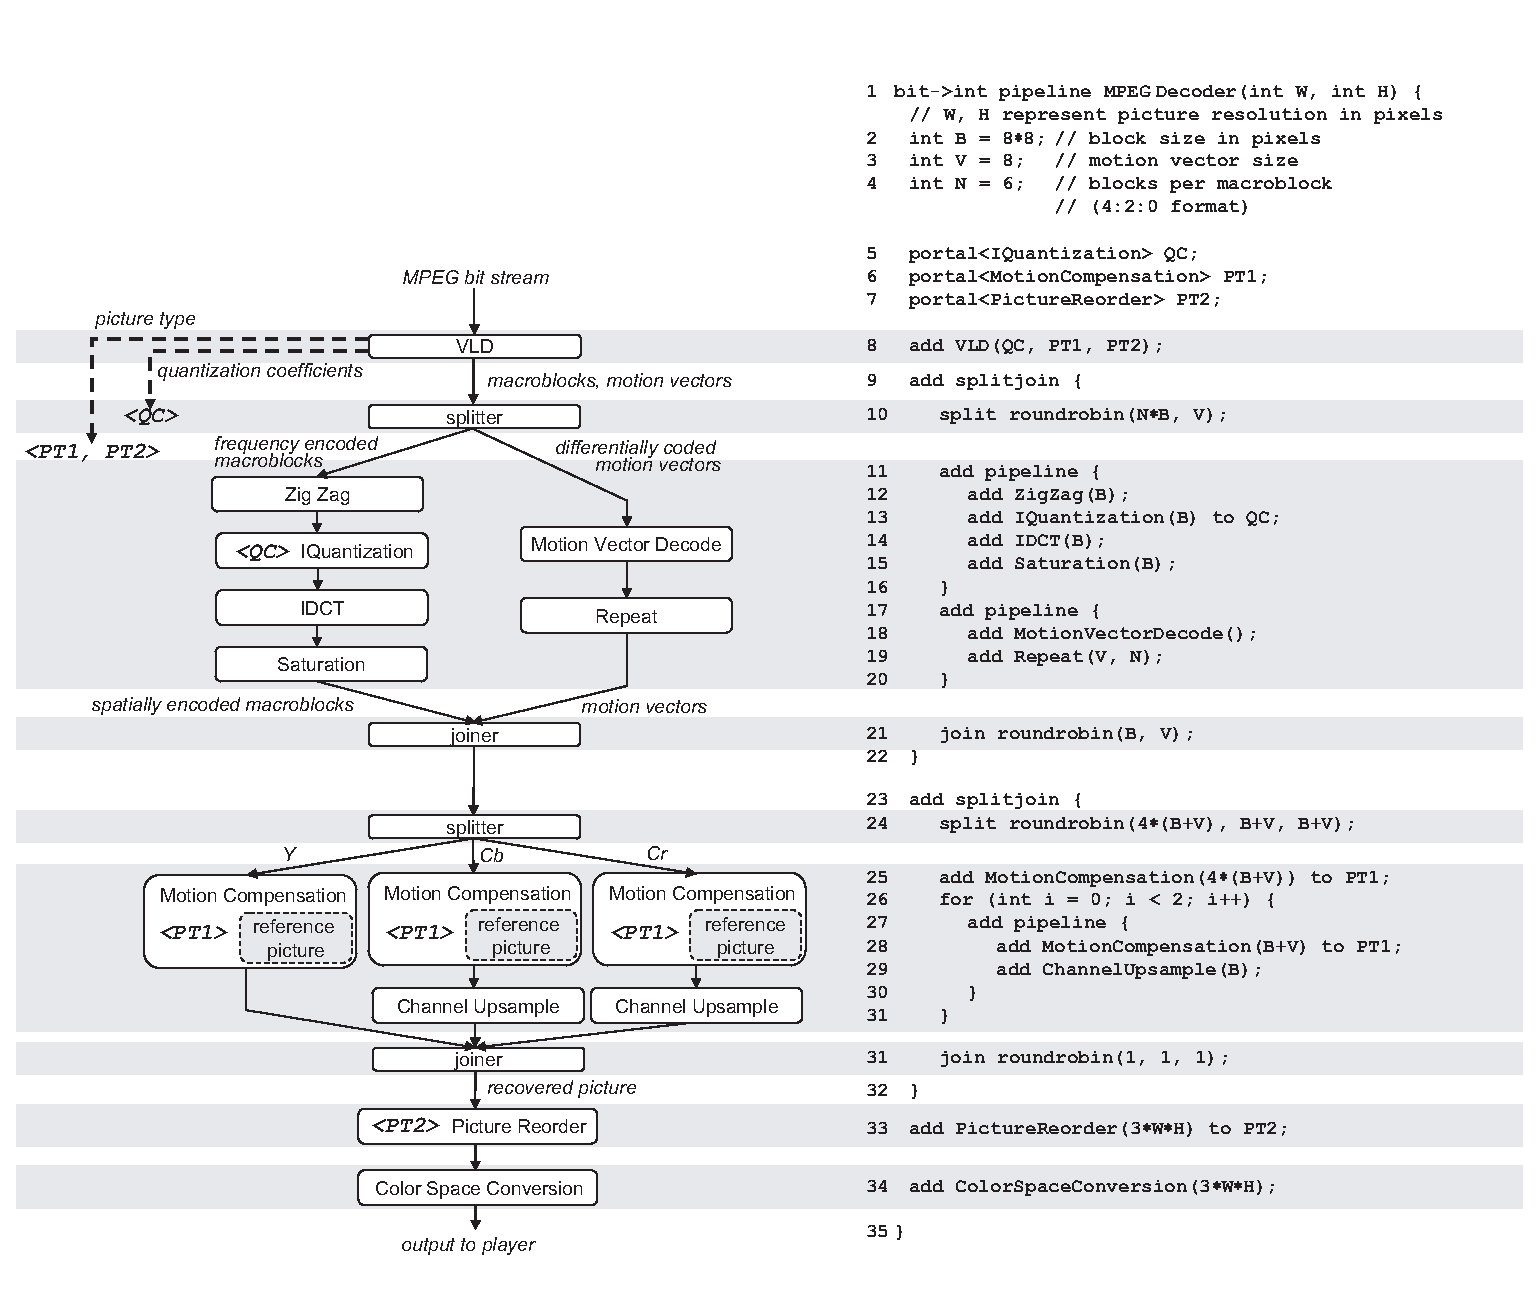
\epsfig{file=decoder_with_code.eps,width=\textwidth}}
%%   \caption{MPEG-2 decoder block diagram and corresponding StreamIt code.}
%%   \label{fig:dec-with-code}
%% \end{figure*}

In StreamIt, all of the processing is encapsulated hierarchically into
single-input, single-output streams with well-defined modular
interfaces. This facilitates development and boosts programmer
productivity, as components can be debugged and verified as standalone
components. The modularity also promotes reuse. For example, the
zig-zag descrambler and inverse DCT can be used as-is in a JPEG decoder.

%%%%
\begin{figure}[h]
  \begin{minipage}{\textwidth}
  \vspace{-1.1in}
  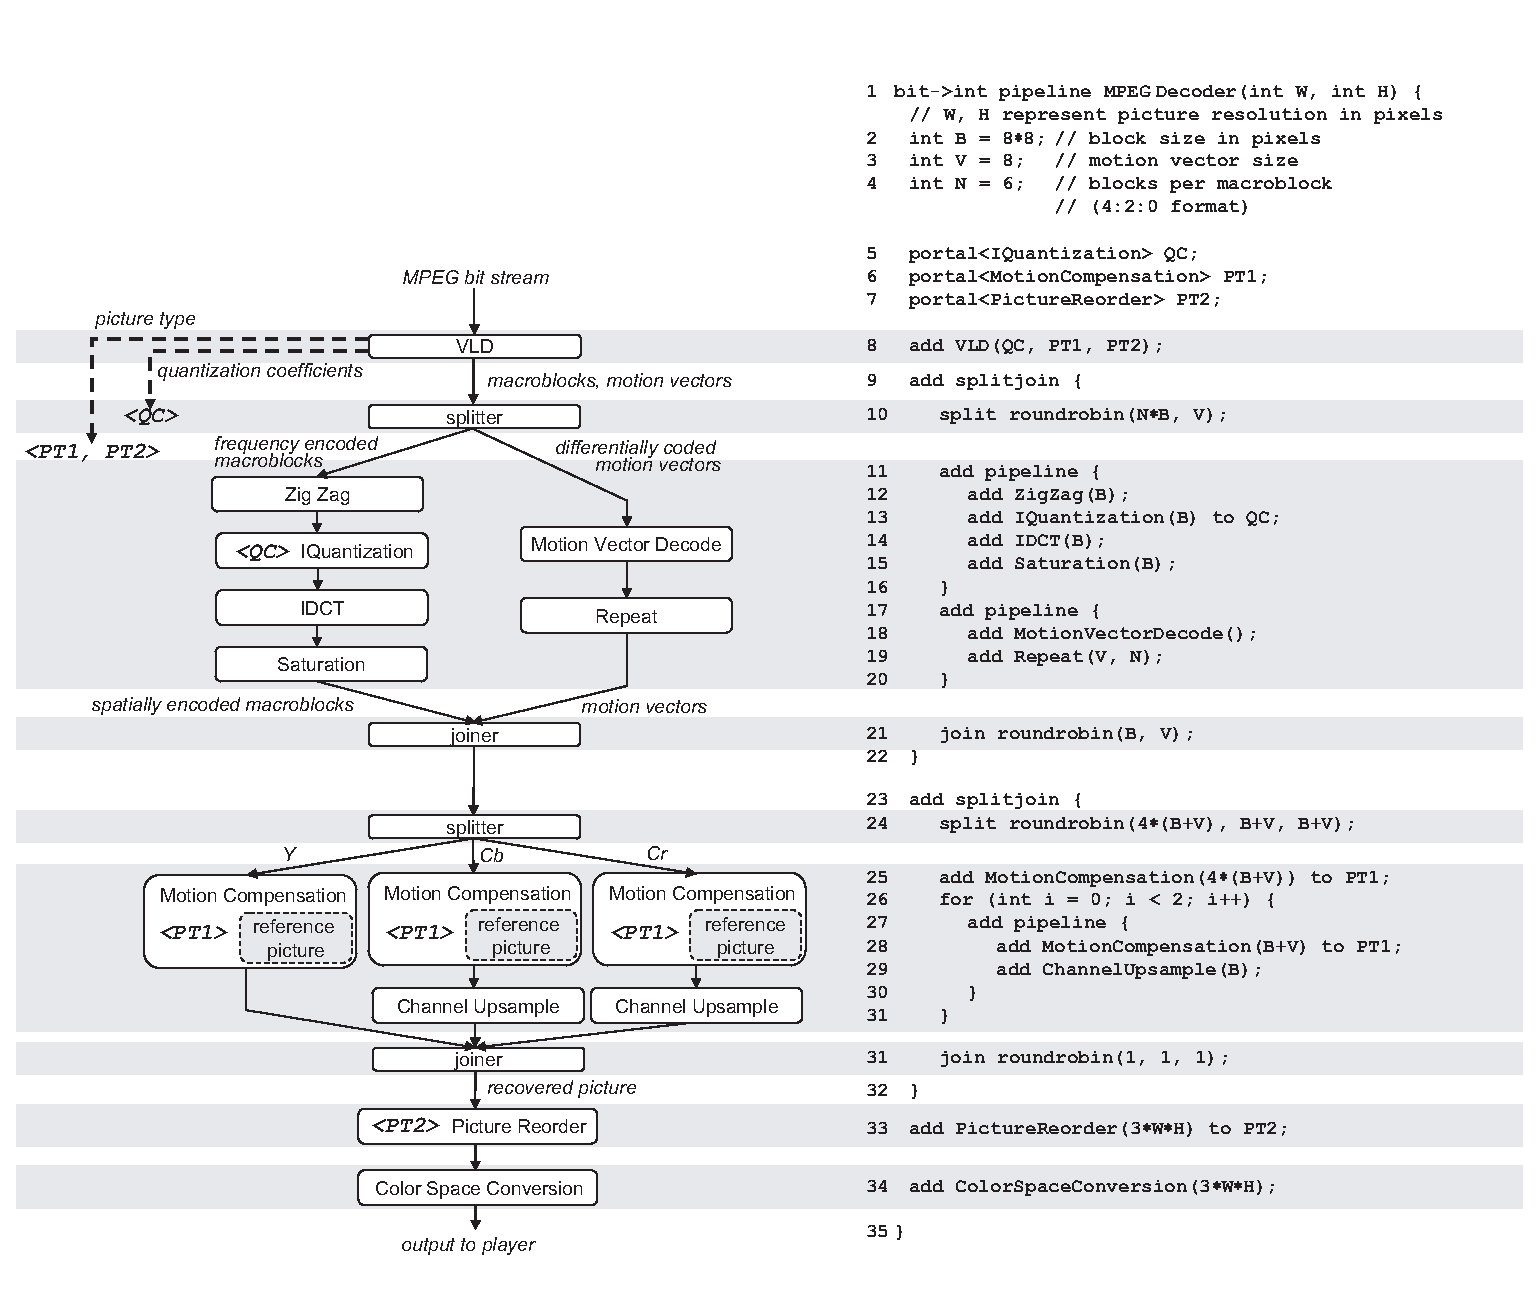
\epsfig{file=decoder_with_code.eps,width=\textwidth}
  \vspace{-22pt}
  \caption{Block diagram of MPEG-2 decoder and corresponding StreamIt code.}
  \vspace{-12pt}
  \label{fig:dec-with-code}
  \end{minipage}
\end{figure}
%%%%

%% \SubSection{Motion Compensation}

% Commented out this section since this information is incorporated into
% the decoder implementation section. - Matt 1/25/06
% An MPEG decoder accepts a bitstream as input and performs Huffman and
% variable run-length decoding (VLD).  This process results in a set of
% quantized, frequency-domain macroblocks and corresponding motion
% vectors.  The decoder inversely quantizes (IQ) the macroblocks and then
% performs an inverse DCT (IDCT) to convert the macroblocks to the
% spatial domain.  For predictively coded macroblocks (e.g., P and B
% pictures), the decoder performs motion compensation (MC) using the
% input motion vectors to find a corresponding macroblock in a
% previously decoded, stored reference picture. This reference
% macroblock is added to the current macroblock to recover the original
% picture data. If the current macroblock is part of an I or P picture,
% then the decoder stores it for future reference.
% Figure~\ref{fig:dec_block} illustrates the decode sequence.

%\begin{figure}[htbp]
%\centerline{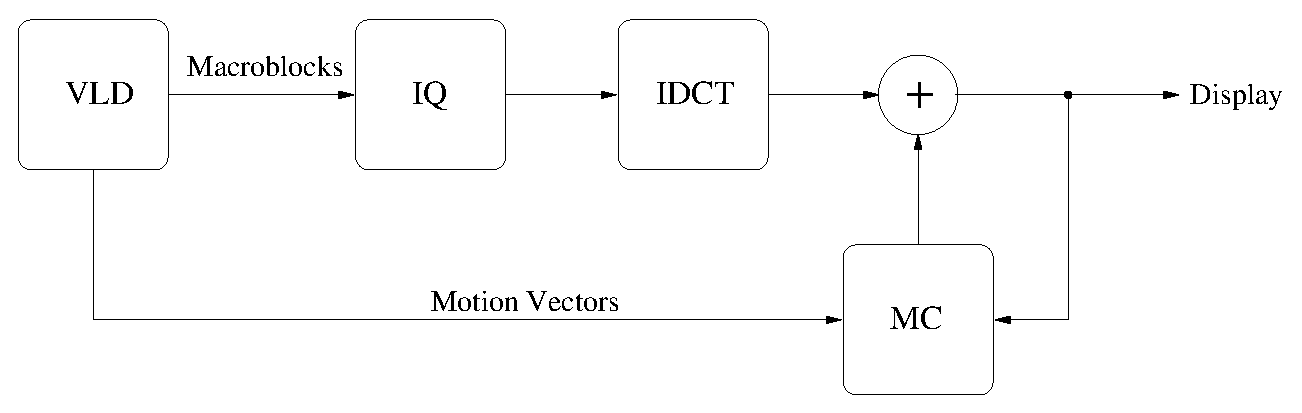
\epsfig{file=dec_block.eps,width=5in}}
%\caption{Block diagram of MPEG-2 decode.}
%\label{fig:dec_block}
%\end{figure}

%% A simple strategy for parallelizing the MPEG-2 decoding can exploit
%% the data parallelism among macroblocks. Using this scheme, the Huffman
%% and run-length decoding is inherently serial, as macroblock boundaries
%% can only be discovered by performing the decode operation.  Once this
%% decode is complete, a parallel implementation can distribute
%% macroblocks to independent streams (using a splitjoin). Each stream
%% performs the inverse quantization, inverse discrete cosine transform,
%% and motion compensation. Furthermore, each stream locally stores
%% reference macroblocks for future motion compensation. Using this
%% strategy, the streams can execute independently with one exception.

%% % TODO: This is the figure showing the macroblock parallelism
%% % I'm not sure where it goes. - Matt
%% \begin{figure*}[t]
%% \vspace{-12pt}
%% %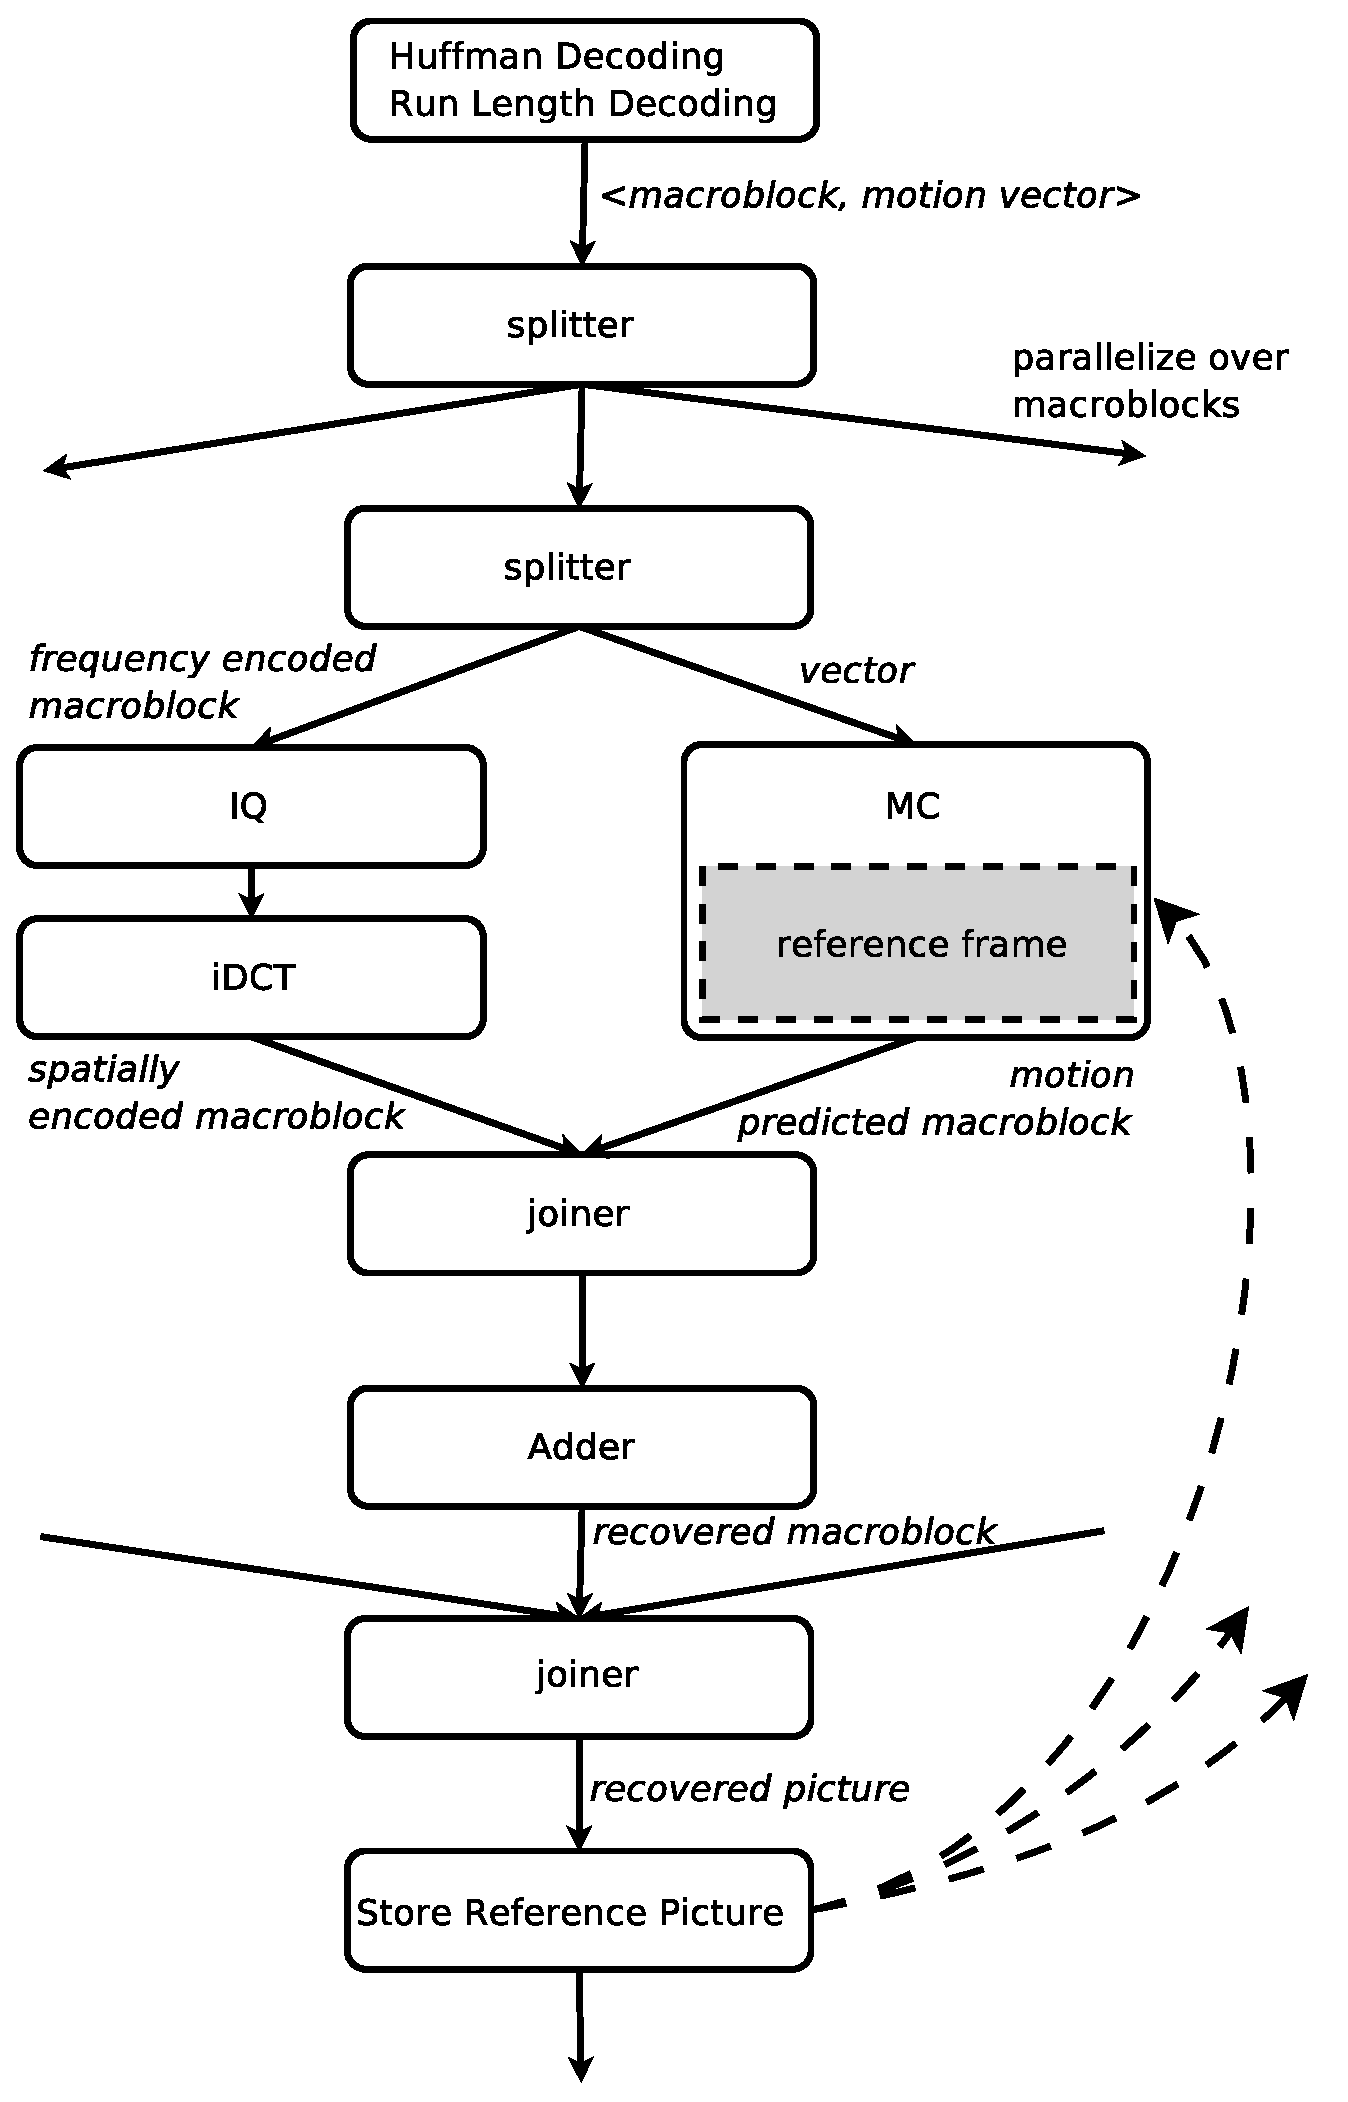
\epsfig{file=decoder_macroblock_parallelism.eps, width=3in}
%% %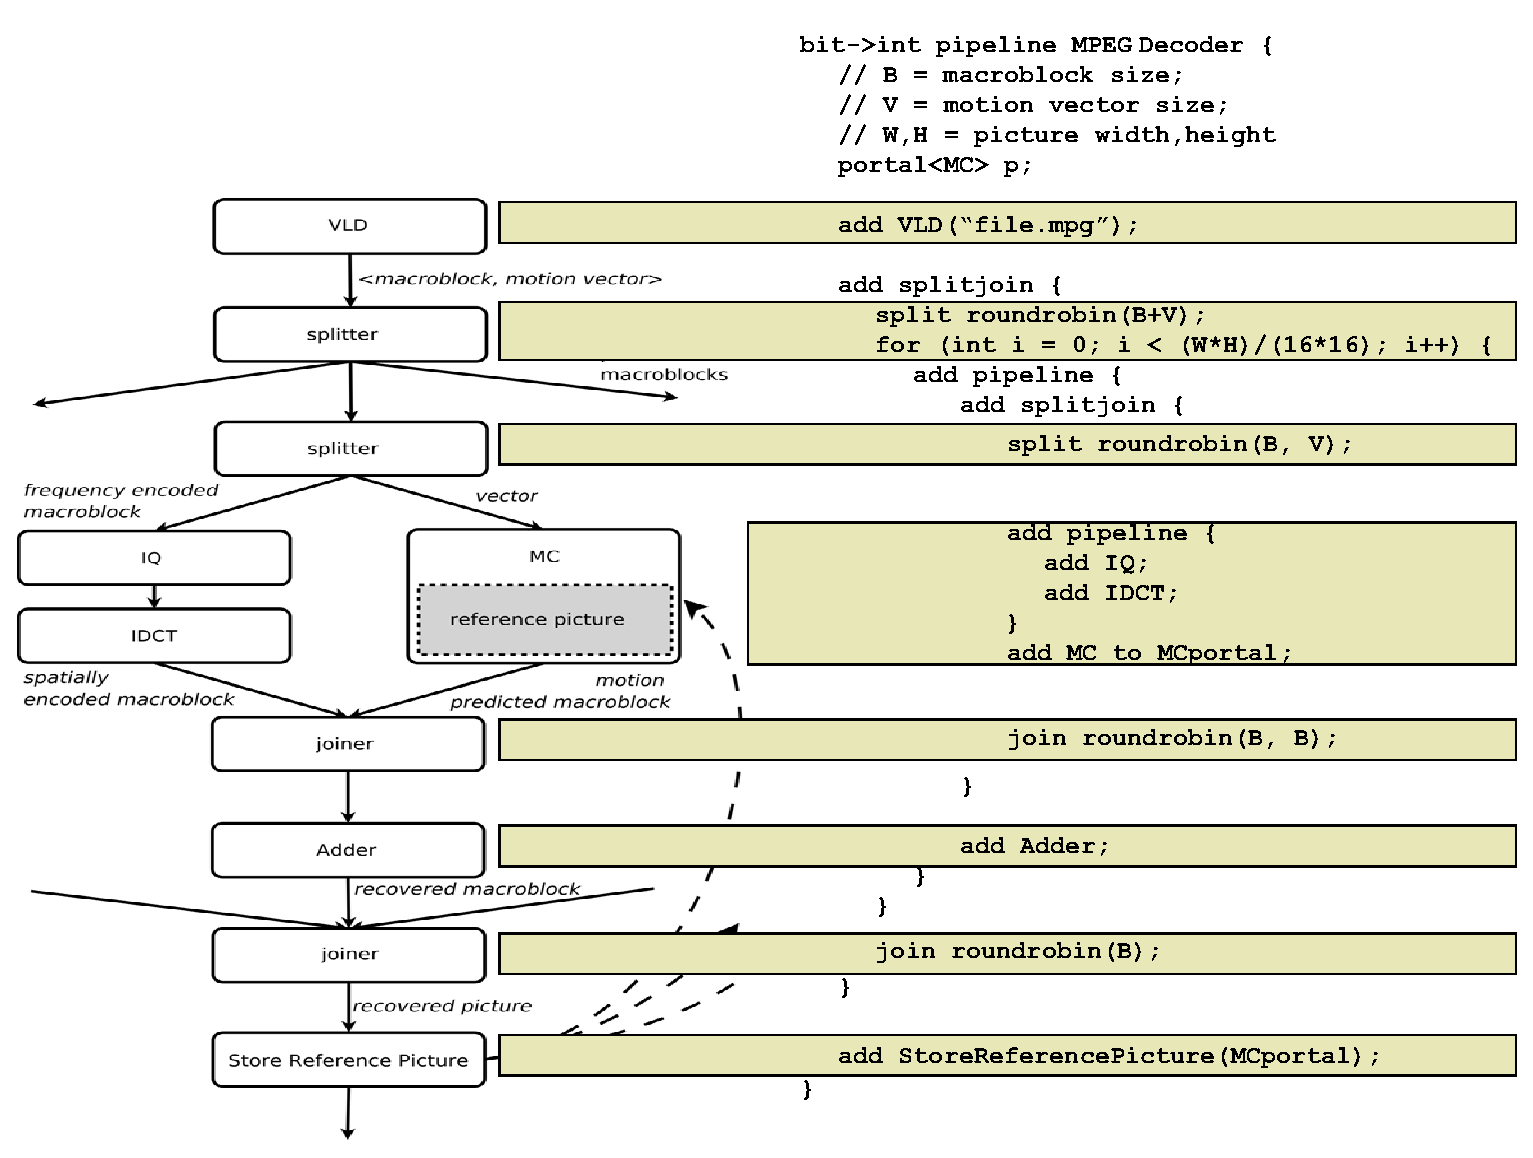
\epsfig{file=decoder-parallel.eps, width=\textwidth}
%% 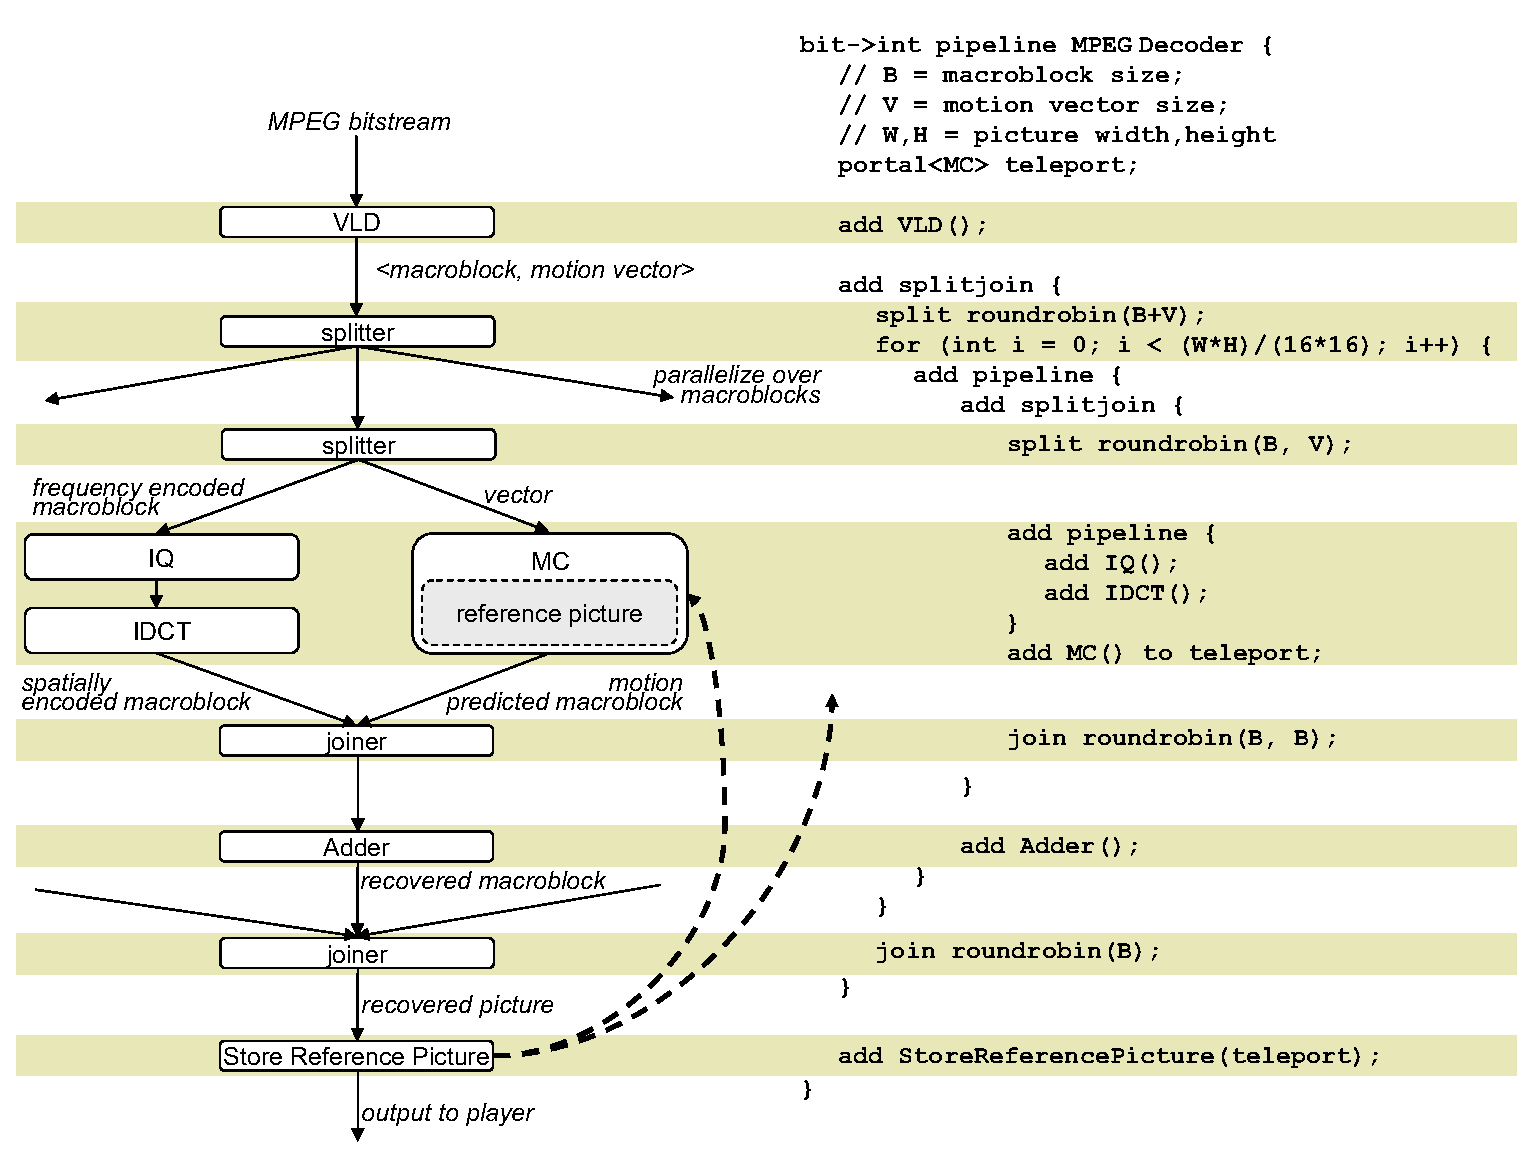
\epsfig{file=decoderpipeline.eps, width=\textwidth}
%% % TODO: Change Matt's 2 am caption.
%% \caption{MPEG-2 decoder exploiting macroblock-level parallelism.}
%% \label{decoder_macroblock_parallelism}
%% \vspace{-6pt}
%% \end{figure*}

%% This exception occurs when a stream is performing motion compensation
%% and the corresponding motion vector indicates a reference macroblock
%% stored in some other stream. In this case, inter-stream communication
%% is required to send the reference data to the requesting stream. This
%% situation is not uncommon, and is more prevalent for higher resolution
%% pictures. A simple scheme for handling this situation is for every
%% stream to broadcast its decoded macroblocks to all other streams. This
%% solution has the benefit of being conceptually easy to understand and
%% implement. StreamIt allows programmers to naturally expose such
%% parallelism.
%% A StreamIt pipeline that operates at macroblock
%% granularity is shown in Figure~\ref{decoder_macroblock_parallelism}. It is
%% worthy to note that there is a high correlation between the stream
%% graph, and the StreamIt syntax describing the pipeline.

%% The implementation can be made more fine grained by exposing the
%% intra-macroblock parallelism. For example, the IQuantization-IDCT
%% pipeline can operate at a block level, rather than at a macroblock
%% granularity. This is easily achieved by encapsulating the  pipeline
%% within a splitjoin to scatter the blocks, operate, and gather the
%% results to recover the parent macroblock.

%% There are many implementation strategies for the decoder, each with
%% varying degrees of exposed parallelism. Of the greatest advantage of
%% the StreamIt implementation is its malleability. The stream graph is
%% easily reconfigured to operate at picture-level granularity (exposing
%% parallelism between chroma channels), macroblock level (exposing even
%% more data-level parallelism), or even at block level (exposing the
%% greatest amount of data-level parallelism).
  \SubSection{Video Sampling Rate}

Macroblocks specify colors using a luminance channel to represent
saturation (color intensity), and two chrominance channels to
represent hue. The human eye is more sensitive to changes in
saturation than changes in hue, so the chrominance channels are
frequently compressed by downsampling the chrominance data within a
macroblock. The type of chrominance downsampling an MPEG-2 encoder
uses is its {\it chrominance format}. The most common chrominance
format is 4:2:0, which uses a single block for each of the chrominance
channels, downsampling each of the two channels from 16x16 to 8x8.  An
alternate chrominance format is 4:2:2. It uses two blocks for each
chrominance channel, downsampling each of the channels from 16x16 to
8x16. The possible chrominance formats are shown in
Figure~\ref{fig:chroma-format}.

To support the 4:2:2 chrominance format in our StreamIt decoder, we
modified 31 lines and added 20 new lines. Of the 31 modified lines, 23
were trivial modifications to pass a variable representing the
chrominance format as a stream parameter. The greatest substantial
change was to the decoding splitjoin previously illustrated in
Figure~\ref{fig:decoding-sj}. In the case of a 4:2:2 sampling rate,
the chrominance data, as it appears on the input tape, alternates
between each of the two chrominance channels. Thus, a a two-tiered
splitjoin is used to properly recover the appropriate chrominance
channels. The new splitjoin is shown in Figure~\ref{fig:chroma-format}.
\begin{figure*}[t]
 \begin{minipage}[t]{4.0in}
   {
    \begin{scriptsize}
    \begin{verbatim} 
    // N = macroblock size + motion vector data size;
    // W = picture width (resolution in pixels);
    // H = picture width (resolution in pixels);

    int->int splitjoin(int chromaFormat) {
      int xUpSample, yUpSample;

      if (chromaFormat == 420) { // 4:2:0 chroma format
        split roundrobin(4*N, 2*N);
        xUpSample = yUpSample = 2;
      } else {                   // 4:2:2 chroma format
        split roundrobin(4*N, 4*N);
        xUpSample = 2;
        yUpSample = 0;
      }

      add LuminanceChannel(W, H, 0, 0, chromaFormat);

      add int->int splitjoin {
        split roundrobin(N, N);
        add ChrominanceChannel(W, H, xUpsample, yUpSample, chromaFormat);
        add ChrominanceChannel(W, H, xUpsample, yupsample, chromaFormat);
        join roundrobin(1, 1);
      }

      join roundrobin(1, 2);
    }
    \end{verbatim}
    \end{scriptsize}
   }
   % \vspace{-3pt}
   \caption{Decoding stream to handle 4:2:0 and 4:2:2 chroma formats.}
   \label{fig:chroma-stream}
  \end{minipage}
  \begin{minipage}[t]{2.0in}
  {
   \begin{center}
    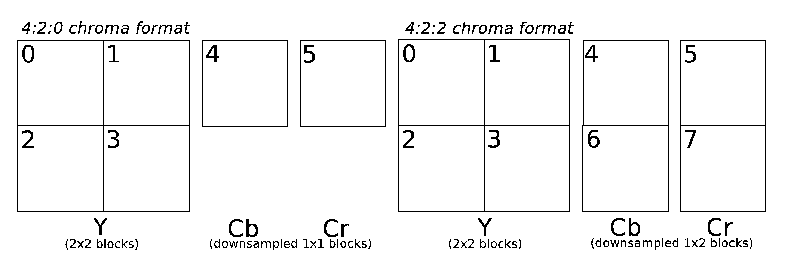
\epsfig{file=chroma_format.eps, width=3in}
    \caption{4:2:0 and 4:2:2 chrominance formats showing macroblock ordering}
    \label{fig:chroma-format}
   \end{center}
  }
  \end{minipage}
\end{figure*}




  %\newcommand{\entry}[1]{\raisebox{0pt}[24pt][20pt]{\parbox{2.75in}{#1}}}
\newcommand{\entrymed}[1]{\raisebox{0pt}[36pt][30pt]{\parbox{2.75in}{#1}}}
\newcommand{\entrybig}[1]{\raisebox{0pt}[42pt][36pt]{\parbox{2.75in}{#1}}}

This section walks through a sample session with the compiler and
runtime system.  We will use the {\tt FMRadio} example from the
StreamIt release as a running example.  To get started, change to the
following directory:
{\small
\begin{verbatim}
% cd $STREAMIT_HOME/apps/examples/cookbook
\end{verbatim}
}
\noindent The example is in {\tt FMRadio.str}. The following
sections describe the compilation of {\tt FMRadio} using the
uniprocessor backend, the Java library, and the Raw backend.  A
summary of the compiler's command-line options can be found in
Appendix~\ref{ap:options}, or by typing {\tt strc -help} at the
command line.

\subsection{Compiling for a Uniprocessor}

There are two ways to compile a StreamIt program for execution on a
general-purpose processor.  Both methods compile StreamIt to a C
program that can be further compiled with a C compiler.  The first
method (the default) preserves the hierarchical structure of the
original program and relies on a C runtime library to do buffer
management.  The second method (``standalone'') produces a
self-contained file where the entire stream graph has been collapsed
into a single function, with buffer management embedded into the code.
The default output is more readable and provides some flexibility (by
exposing the runtime library interface).  The standalone output might
be useful for groups interested in compiling C programs to new
architectures; however, the size of the main work function might grow
very large.  We recommend using the default backend with the C runtime
library.

\medskip {\bf Compiling for C library.}  To compile {\tt FMRadio} using the
uniprocessor backend and C runtime library, issue the following
command (the compiler output is shown): {\small
\begin{verbatim}
% strc FMRadio.str -o fm
Running Constant Prop and Unroll... done.
Raising variable declarations... done.
Propagating constant fields... done.
Flattening blocks... done.
Raising variables... done.
Raising variable declarations... done.
Moving initial assignments... done.
Structuring... done.
Scheduling... got schedule, interpreting... done.
Annotating IR for uniprocessor... done.
Generating code...
\end{verbatim}
} 
This will create a C file named FMRadio.c and a binary named {\tt
fm}.  The binary can be executed for 5 steady-state iterations as follows:
{\small
\begin{verbatim}
% ./fm -i 5
278074.000000
278074.750000
278075.437500
278075.968750
278076.437500
\end{verbatim}
} 
During the compilation process, several {\tt dot} graphs are
generated.  The {\tt dot} format can be displayed and converted to
other formats using the Graphviz software, which is available
online\footnote{\tt http://www.research.att.com/sw/tools/graphviz/}.
For example, we can examine a stream graph for the FM application as
follows: {\small
\begin{verbatim}
% dotty first-sir-tree.dot
\end{verbatim}
} The result appears in Figure~\ref{fig:fm-sir-tree}.  A complete list
of the {\tt dot} graphs that are produced on the normal uniprocessor path
are shown in Figure~\ref{fig:dot-uni}.

\begin{figure}[t]
\hspace{-0.75in}\psfig{figure=fm-sir-tree.eps,width=6.6in}
\caption{{\tt first-sir-tree.dot} for the FMRadio example.\protect\label{fig:fm-sir-tree}}
\end{figure}

\begin{figure}[t]
{\small
\noindent \begin{tabular}{|l|l|}
\hline
{\bf Filename} & {\bf Description} \\
\hline
{\tt first-sir-tree.dot} & \entry{Original stream graph, as written by programmer.} \\ \hline
{\tt before-partition.dot} & \entry{Canonical version of stream graph, before any stream transformations are applied.  Nodes are annotated with their I/O rates.}\\ \hline
{\tt after-partition.dot} & \entry{Canonical version of stream graph, after any stream transformations are applied.  Nodes are annotated with their I/O rates.}\\ \hline
{\tt schedule.dot} & \entry{Final stream graph, annotated with I/O rates and the number of times each node executes in the initial and steady-state schedule.} \\ \hline
\end{tabular}
}
\caption{{\tt dot} graphs produced on the uniprocessor path.\protect\label{fig:dot-uni}}
\end{figure}

\medskip {\bf Domain-specific optimizations.}  It turns out that our
version of the FMRadio has a lot of redundant computation the way in
which it is written.  For example, each {\tt BandPassFilter} could be
implemented as a single FIR filter rather than a composition of {\tt
LowPassFilter}'s; in fact, the entire equalizer could be collapsed to
a single FIR filter.  Further, some of these operations are more
efficient if executed in the frequency domain, with an FFT/IFFT being
used to translate to and from the time domain.

The StreamIt compiler includes a set of domain-specific optimizations
that will automatically perform the transformations described above.
The analysis considers all filters that are ``linear''---that is, each
of their outputs is an affine combination of their inputs.  The
compiler automatically detects linear filters by analyzing the code in
their work functions.  Then, it performs algebraic simplification of
adjacent linear filters, as well as automatic translation to the
frequency domain.  Since these transformations can sometimes hamper
performance, the compiler also does a global cost/benefit analysis to
determine the best set of transformations for a given stream graph.

\begin{figure}[t]
\hspace{3pt} \psfig{figure=fm-linear-simple.eps,width=4.6in}
\caption{{\tt linear-simple.dot}, which illustrates the linear sections of FMRadio.  Linear filters are shaded blue, while linear containers are shaded pink.\protect\label{fig:fm-linear-simple}}
\end{figure}

\begin{figure}[t]
\vspace{-6pt}
\begin{center}
\mbox{}\psfig{figure=fm-after-linear.eps,width=2.5in}
\vspace{-6pt}
\caption{Final stream graph ({\tt after-linear.dot}) for the FMRadio, compiling with the {\tt -linearpartition} option.\protect\label{fig:fm-after-linear}}
\end{center}
\vspace{-14pt}
\end{figure}

The {\tt linearpartition} option to strc will enable linear analysis
and optimizations\footnote{In contrast, the {\tt linearreplacement}
and {\tt frequencyreplacement} options will perform maximal algebraic
simplification and frequency translation, respectively, even in cases
where it is not beneficial.}:
{\small
\begin{verbatim}
% strc -linearpartition FMRadio.str -o fm
Running Constant Prop and Unroll... done.
Raising variable declarations... done.
Propagating constant fields... done.
Flattening blocks... done.
Raising variables... done.
Raising variable declarations... done.
Moving initial assignments... done.
Running linear analysis...
WARNING: Assuming method call expression non linear(atan). Also 
  removing all field mappings.
WARNING: Insufficient pushes detected in filter
done with linear analysis.
Linear partitioner took 1 secs to calculate partitions.
Structuring... done.
Scheduling... got schedule, interpreting... done.
Annotating IR for uniprocessor... done.
Generating code...
\end{verbatim}
} 
%
The linear analysis produces its own set of {\tt dot} files that we
can use to inspect the results of the optimizations.  For example, the
following command will display the stream graph with the linear
sections highlighted: {\small
\begin{verbatim}
% dotty linear-simple.dot
\end{verbatim}
} 
%
As shown in Figure~\ref{fig:fm-linear-simple}, FMRadio contains many
linear components, including the first LowPassFilter and the
equalizer.  To see the stream graph after linear optimizations have
been applied, we can issue the following command:
{\small
\begin{verbatim}
% dotty after-linear.dot
\end{verbatim}
} 
%
As illustrated in Figure~\ref{fig:fm-after-linear}, this stream
graph shows that the equalizer was collapsed into a single filter and
then was translated to the frequency domain (by virtue of the ``Freq''
prefix in the filter's name.)  However, the LowPassFilter at the top
was left unmodified; this is because it has a large pop rate that
degrades the performance of the frequency transformation.  In this
case, the linear optimizations lead to a 6.5X improvement in
throughput.

The linear optimizations produce additional {\tt dot} graphs; see
Figure~\ref{fig:dot-linear} for details.  For more information on the
linear analysis and optimization, please refer to {\tt http://cag.lcs.mit.edu/linear}.

\begin{figure}[t]
\vspace{-6pt}
{\small
\noindent \begin{tabular}{|l|l|}
\hline
{\bf Filename} & {\bf Description} \\
\hline
{\tt ldp-partition-input.dot} & \entry{The stream graph as it was input to the linear partitioning algorithm.}\\ \hline
{\tt linear.dot} & \entry{The stream graph with linear filters highlighted and each node annotated with its I/O rates.}\\ \hline
{\tt linear-simple.dot} & \entry{Same as {\tt linear.dot} but without the I/O rates.}\\ \hline
{\tt after-linear.dot} & \entry{The stream graph after linear transformations are complete.} \\ \hline
\end{tabular}
}
\vspace{-5pt}
\caption{{\tt dot} graphs produced by linear optimizations.\protect\label{fig:dot-linear}}
\vspace{-5pt}
\end{figure}

\bigskip {\bf Compiling as standalone.}  To compile FMRadio to a
standalone file that can execute without the C runtime library, use
the {\tt -standalone} option:
{\small
\begin{verbatim}
% strc -standalone FMRadio.str -o fm
/*
Out of Kopi2SIR.
Out of semantic checker.
*/
Entry to RAW Backend
Moving initializers into init functions... done.
Running Constant Prop and Unroll...
Done Constant Prop and Unroll...
Running Constant Field Propagation...
Done Constant Field Propagation...
Running Partitioning...
  Found 26 tiles.
  Building stream config...
  Calculating partition info...
  Tracing back...
  Work Estimates:
    Fused_Flo_Low_FMD_Low_Pre_E...      10240   (100%)
Done Partitioning...
Flattener Begin...
Filters in Graph: 1
Flattener End.
Simulated Annealing Assignment
Tiles layout.assigned: 1
Initial Cost: 0.0
Assign End.
Switch Code Begin...
FineGrainSimulator Running...
End of init simulation
End of steady-state simulation
sw0.s written
Switch Code End.
Generating Raw Code: 
  Fused_Flo_Low_FMD_Low_Pre_EqS_Pos_Fil_Flo_172 (no buffer)
Tile Code begin...
Optimizing Fused_Flo_Low_FMD_Low_Pre_EqS_Pos_Fil_Flo_172...
Code for Fused_Flo_Low_FMD_Low_Pre_EqS_Pos_Fil_Flo_172 
  written to tile0.c
Tile Code End.
Creating Makefile.
Exiting
\end{verbatim}
} 
%
As is evident in the compiler output above, the standalone option
utilizes the Raw backend and stores the self-contained output file in
{\tt tile0.c} (as well as the binary {\tt fm}).  Also, due to an
implementation detail, it is not possible to control the number of
runtime iterations for standalone programs (they will run forever.)

\subsection{Using the Java Library}

A convenient aspect of the StreamIt compilation toolchain is that all
StreamIt programs are first translated to Java files that can be
executed against a Java runtime library using a normal Java Virtual
Machine.  This is especially useful for testing and debugging
applications, as well as validating the output of the compiler.

The library can be invoked with the {\tt -library} flag.  Since {\tt
strc} will both compile and execute the file in the library, you can
specify the number of iterations to execute with the {\tt -i} flag.
For example, to compile FMRadio and run for 5 iterations in the
library, do as follows\footnote{In this case, the library's output is
marginally different from the compiler's due to numerical precision
issues.}:
%
{\small
\begin{verbatim}
% strc -library -i 5 FMRadio.str
278073.94
278074.75
278075.38
278075.94
278076.4
\end{verbatim}
} 
%
You can also inspect the {\tt FMRadio.java} file, which was generated
for execution in the library.  It can be compiled and run with a
standard Java compiler and JVM.  The library also produces a {\tt dot}
graph of the program; it is given the same name as the StreamIt file,
but with a {\tt dot} extension ({\it i.e.,} it is {\tt FMRadio.dot} in
this case.)

There are a few additional options available in the library.  For
instance, you can direct the library not to execute the program, but
to instead just print the schedule of filter firings:
{\small
\begin{verbatim}
% strc -library -norun -printsched FMRadio.str
init = [
$0 = FloatOneSource@3541984.work
$1 = LowPassFilter@4565111.work
$2 = FMDemodulator@1233730.work
$3 = EqSplit@4689495.duplicate
$4 = BPFCore@6288523.duplicate
$5 = BPFCore@4074853.duplicate
$6 = BPFCore@5058143.duplicate
$7 = BPFCore@2951274.duplicate
$8 = { {379 $0} {64 $1} {63 $2} {63 $3} 
       {63 $4} {63 $5} {63 $6} {63 $7} }
]
steady = [
$9 = LowPassFilter@3738425.work
$10 = LowPassFilter@1042371.work
$11 = BPFCore@6288523.roundrobin
$12 = Subtracter@3144816.work
$13 = EqSplit$2@6700605.work
$14 = LowPassFilter@5188736.work
$15 = LowPassFilter@7510100.work
$16 = BPFCore@4074853.roundrobin
$17 = Subtracter@1467553.work
$18 = EqSplit$2@2671847.work
$19 = LowPassFilter@503498.work
$20 = LowPassFilter@6589979.work
$21 = BPFCore@5058143.roundrobin
$22 = Subtracter@2069821.work
$23 = EqSplit$2@8316668.work
$24 = LowPassFilter@1649037.work
$25 = LowPassFilter@7808535.work
$26 = BPFCore@2951274.roundrobin
$27 = Subtracter@230849.work
$28 = EqSplit$2@4354460.work
$29 = EqSplit@4689495.roundrobin
$30 = Equalizer$1@3615258.work
$31 = FloatPrinter@2964388.work
$32 = { {5 $0} $1 $2 $3 $4 $9 $10 $11 $12 $13 $5 $14 $15 $16 $17 $18
        $6 $19 $20 $21 $22 $23 $7 $24 $25 $26 $27 $28 $29 $30 $31 }
]
!ml sched size = 39
!ml buff size = 1299
\end{verbatim}
%$
} 
%
Currently, the default scheduler is a minimal latency scheduler that
uses phases to compress the code size.  The schedule listed above has
two components: an initialization schedule (to initialize buffers for
filters that peek) and a steady-state schedule (that can loop
infinitely).  Each filter and splitter in the graph is given a number
for easy reference, and then the schedule is printed at the bottom.  A
loop nest in the schedule is denoted by {\tt (N F)}, where the filter
{\tt F} executes {\tt N} times.  The schedule size and buffer size
required are printed at the end of the listing.

Additional options for the library can be found in
Appendix~\ref{ap:options}.

\subsection{Compiling for Raw}

To compile for an {\tt NxN} Raw machine, use the {\tt -raw N}
option\footnote{You can also compile for an NxM machine by using {\tt
-raw N -rawcol M}.}.  In most cases, you will want to use {\tt -raw
4}, since the actual chip has 4 tiles on each side.  When compiling to
Raw, we also recommend using the {\tt -O1} flag to enable common
optimizations; the default is {\tt -O0} (no optimizations), and the
most aggressive is {\tt -O2} (which includes slow and potentially
unstable transformations).  More information about specific
optimizations can be found in Appendix~\ref{ap:options}.

Compiling FMRadio looks like this: {\small
\begin{verbatim}
% strc -raw 4 -O1 FMRadio.str
/*
Out of Kopi2SIR.
Out of semantic checker.
*/
Entry to RAW Backend
Moving initializers into init functions... done.
Running Constant Prop and Unroll...
Done Constant Prop and Unroll...
Running Constant Field Propagation...
Done Constant Field Propagation...
Running Partitioning...
  Found 26 tiles.
  Building stream config...
  Calculating partition info...
  Tracing back...
  Work Estimates:
    LowPassFilter__24                   1444    (10%)
    LowPassFilter__59                   1420    (10%)
    LowPassFilter__80                   1420    (10%)
    LowPassFilter__59                   1420    (10%)
    LowPassFilter__80                   1420    (10%)
    LowPassFilter__59                   1420    (10%)
    LowPassFilter__80                   1420    (10%)
    LowPassFilter__59                   1420    (10%)
    LowPassFilter__80                   1420    (10%)
    Fused_Pre_EqS_Pos_Fil_Flo           386     (2%)
    FMDemodulator__38                   224     (1%)
    FMDemodulator__38                   224     (1%)
    FloatOneSource__3                   110     (0%)
Done Partitioning...
Flattener Begin...
Filters in Graph: 13
Flattener End.
Simulated Annealing Assignment
Tiles layout.assigned: 15
Initial Cost: 60060.0
Final Cost: 29055.0 Min Cost : 21119.0 in  451 iterations.
Assign End.
Cannot perform Rate Matching.
Switch Code Begin...
WorkBasedSimulator Running...
End of init simulation
End of steady-state simulation
sw0.s written
\end{verbatim}
$\dots$
\begin{verbatim}
sw14.s written
Switch Code End.
Generating Raw Code: FloatOneSource__3_96 (Direct Communication)
\end{verbatim}
$\dots$
\begin{verbatim}
Generating Raw Code: FMDemodulator__38_178 (simple)
Tile Code begin...
Optimizing FloatOneSource__3_96...
Code for FloatOneSource__3_96 written to tile0.c
\end{verbatim}
$\dots$
\begin{verbatim}
Optimizing FMDemodulator__38_178...
Code for FMDemodulator__38_178 written to tile2.c
Code  written to tile10.c
Tile Code End.
Creating Makefile.
Exiting
\end{verbatim}
} 
%

\begin{figure}[t]
\hspace{0.25in}\psfig{figure=fm-after-partition.eps,width=4.6in}
\caption{\protect\small Load-balanced stream graph ({\tt after-partition.dot}) that is output by partitioner for executing FMRadio on a 4x4 Raw machine.\protect\label{fig:fm-after-partition}}
\end{figure}

\begin{figure}[t]
{\small
\noindent \begin{tabular}{|l|l|}
\hline
{\bf Filename} & {\bf Description} \\
\hline
{\tt dp-partition-input.dot} & \entry{The stream graph in the format used by the partitioning algorithm.}\\ \hline
{\tt work-before-partition.dot} & \entrybig{The stream graph before partitioning, annotated with estimates of the steady-state work within each node.  Nodes with the same amount of work are given the same color (although the colors themselves are meaningless.)}\\ \hline
{\tt work-before-partition.txt} & \entry{Text listing of the work estimates for filters in the graph, before load balancing.}\\ \hline
{\tt work-after-partition.dot} & \entry{The stream graph after partitioning, annotated with work estimates as above.}\\ \hline
{\tt work-after-partition.txt} & \entry{Text listing of the work estimates for filters in the graph, after load balancing.}\\ \hline
{\tt flatgraph.dot} & \entry{The stream graph with structure eliminated, before it is mapped onto Raw.} \\ \hline
{\tt layout.dot} & \entrymed{The final layout of filters onto Raw tiles, with arrows between communicating filters.  Note that the arrows do NOT indicate the routes that items take.}\\ \hline
{\tt initial-layout.dot} & \entry{The initial layout, before the simulated annealing algorithm.} \\ \hline
\end{tabular}
}
\caption{Files produced by the Raw backend, above and beyond those produced by the uniprocessor backend.\protect\label{fig:dot-raw}}
\end{figure}

A number of {\tt dot} files are produced during the compilation to
Raw; they are listed in Figure~\ref{fig:dot-raw}.  For example, since
there are more filters than Raw tiles, the compiler has to partition
the graph into a set of load-balanced execution units.  The output of
the partitioning stage can be viewed as follows (see
Figure~\ref{fig:fm-after-partition}): 
%
{\small
\begin{verbatim}
% dotty after-partition.dot
\end{verbatim}
} 
%
In this case, the partitioner detected that the LowPassFilter's in the
equalizer were on the critical path, so it allocated a tile for each
one.  The bottom part of the equalizer was fused with the end of the
pipeline.  Also, the FMDemodulator was fissed into two data-parallel
sections.  The steady-state work estimates for before and after
partitioning can be found in {\tt work-} {\tt before-partition.dot}
and {\tt work-after-partition.dot}.  There are also corresponding text
files.

After partitioning, the compiler maps the partitioned stream graph to
the Raw tiles.  The layout can be viewed in {\tt layout.dot}: 
%
\clearpage
%
{\small
\begin{verbatim}
% dotty layout.dot
\end{verbatim}
} 
\begin{figure}[t]
\psfig{figure=fm-layout.eps,width=4.6in}
\caption{\protect\small Final layout ({\tt layout.dot}) for the FMRadio on a 4x4 Raw machine.\protect\label{fig:fm-layout}}
\end{figure}
%
This layout is shown in Figure~\ref{fig:fm-layout}.  Note that the
arrows represent communication channels between filters, but are
unrelated to the routes assigned for these channels.

The final outputs of the Raw backend are: 1) the tile code, which runs
on the compute processors ({\tt tile*.c}), 2) the switch code, which
routes items between processors ({\tt sw*.s}), and 3) {\tt
Makefile.streamit}, which interfaces with the Raw simulation
infrastructure and orchestrates the execution.

\bigskip {\bf Using the Raw simulator.}  To execute the output of the
Raw backend, you will need the Raw simulator and ``starsearch''
infrastructure; for more information, see the Raw website at {\tt
http://cag.lcs.mit.edu/raw}.  The StreamIt compiler makes use of the
cycle-accurate BTL (``Beetle'') simulator for Raw.

To run the simulator, do as follows:
\begin{verbatim}
make -f Makefile.streamit run
\end{verbatim}

This command will cause the simulator to boot up, execute the startup
code and then run for a bunch of cycles. If you want to quit before
the simulation is done, use CTL-C.

Once the simulator is executing the program, the output should should
look as follows:
{\small
\begin{verbatim}
[31: 00001384b]: 278073.937500
[31: 000013d53]: 278074.750000
[31: 000013fc4]: 278075.375000
[31: 000014278]: 278075.937500
[31: 0000144e4]: 278076.406250
[31: 000014798]: 278076.812500
[31: 000014a04]: 278077.156250
[31: 000014cb8]: 278077.468750
[31: 000014f24]: 278077.750000
[31: 0000151d8]: 278078.000000
...
\end{verbatim}
}
The first number (31) represents the fact that the tile at row 3,
column 1 issued the print command. The next number ({\it e.g.},
00001384b) is the cycle count (in hexadecimal) at which the third
number was produced. The third number is the output value that is
produced from FMRadio.

\medskip {\it Running in debug mode.} To run the simulator in interactive debug
mode, you should run:
\begin{verbatim}
make -f Makefile.streamit debug
\end{verbatim}
This will change the terminal window to a text layout of the Raw
tiles being executed, showing the active instruction stream of each.
An extra ``shunt'' window will appear to control the actions of the
debugger; it will look something like this:
{\scriptsize
\begin{verbatim}
// welcome to beetle
// try: 
  help(); help(``help'');

Configuration: 

[THREAD_C THREAD_E DEVICE NAME    RESET ROUTINE          CALC ROUTINE           
PARAM   ]

[081c0f10 00000000 Serial Rom     dev_serial_rom_reset   dev_serial_rom_calc    
0844c9d0]
[0815fcf0 00000000 Print Service  dev_print_service_rese dev_print_service_calc 
0844c410]
\end{verbatim}
$\dots$
\begin{verbatim}
[08205508 00000000 streaming_dram dev_streaming_dram_res dev_streaming_dram_cal 
08444220]

// Use VMShowPositionOfThread(THREAD #); to inspect execution of device 

/*[0] 0*/ 
\end{verbatim}
}

To start the simulator, type {\tt go();}.  This will boot up the Raw
processor, bring the program into memory, and perform some other
initialization tasks.  After initialization, there will be a message
and a prompt such as:
{\small
\begin{verbatim}
running...
\end{verbatim}
$\dots$
\begin{verbatim}
### PASSED: -0000000001 ffffffff      nan [x,y] = [1, 3]
// [ serial rom : finished 
     tile.B79414E0.0004-0004.rbf-15 --> static port 15 ]
// *** interrupted [135033/inf]
stopped.
/*[34576982] 2*/ 
\end{verbatim}
}

You are now ready to start doing useful things with the debugger.  The
following are the most useful commands:

\begin{itemize}

\item {\bf go();} starts the simulator executing, without any limit as
to how many cycles it will run.

If you want to stop the simulator, you can hit CTL-C in the main
window (not the shunt window), which will give you the command prompt
back in the shunt window.

\item {\bf step(N);} steps the simulator forward \texttt{N} cycles. At
the end of {\tt N} cycles, the simulator will stop executing and
return you to a command prompt.

By stepping the simulator \texttt{N} cycles, each processor (of the
16) is stepped forward \texttt{N} cycles.

\item {\bf sv(N);} produces a graphical execution trace over {\tt N}
cycles.  This trace shows the activity of each processor over time; we
call it a ``bloodgraph'' because red indicates that a processor is
blocked and performing no useful work.  For FMRadio, the result of
running {\tt sv(10000);} appears in Figure~\ref{fig:fm-bloodgraph}.

\clearpage

\begin{figure}[t]
\begin{center}
\hspace{0pt}\psfig{figure=fm-bloodgraph.eps,width=4.5in}
\caption{\protect\small Execution trace for FMRadio on a 4x4 Raw
machine.  The vertical axis represents processors, while the
horizontal axis represents time.  Note that the entirely white
processor is not being used by the configuration (you can verify this
by inspecting {\tt layout.dot}, which shows the tile to be
empty).\protect\label{fig:fm-bloodgraph}}
\end{center}
\end{figure}

The complete guide to the colors in the bloodgraph is as follows: \vspace{6pt}

\begin{tabular}{|l|l|}
\hline
{\bf Color} & {\bf Meaning} \\
\hline
{\tt white} & useful work\\ \hline
{\tt purple} & floating point operation\\ \hline
{\tt green} & pipeline stall, {\it e.g.,} for a hazard\\ \hline
{\tt blue} & blocked while receiving an item from the switch\\ \hline
{\tt red} & blocked while sending an item to the switch\\ \hline
\end{tabular}

\item {\bf quit();} will exit the interactive debugger.  Incidentally,
typing CTL-D will close the shunt window.

\end{itemize}

{\it The cycle limit.}  By default, there is a limit on the number of
cycles that the simulator will execute before halting (so as not to
freeze scripts, etc., with an infinite loop.)  If you run the
simulator and it finishes before your program produces any outputs,
you can edit {\tt Makefile.streamit} and delete the lines which define
{\tt LIMIT} and {\tt SIM-CYCLES}.  Then the simulator will run
indefinitely.

\bigskip {\bf Gathering numbers.}  The compiler provides automatic
support for gathering throughput, MFLOPS, and utilization numbers, as
well as automated generation of bloodgraphs.  To collect these
performance statistics, use the {\tt -numbers} option, which takes an
argument indicating the number of steady-state cycles to execute:
{\small
\begin{verbatim}
% strc -raw 4 -O1 -numbers 15 FMRadio.str
\end{verbatim}
} 
%
Compilation will proceed as before, except that the code will be
instrumented to gather numbers using hooks in the Raw simulator.  The
program should then be executed in batch mode, and number gathering
messages (one per steady-state) will replace the standard output: 
%
{\small
\begin{verbatim}
% make -f Makefile.streamit run
\end{verbatim}
$\dots$
\begin{verbatim}
running...

### PASSED:  1073741901 4000004d      2.00001836 [x,y] = [0, 0]

### PASSED: -0000000001 ffffffff             nan [x,y] = [0, 0]
Interrupted tile 0, pc = 0x3b8
stopped.
running...
Cycles: 1312,  MFLOPS: 463
Cycles: 1312,  MFLOPS: 463
Cycles: 1312,  MFLOPS: 463
Cycles: 1312,  MFLOPS: 464
Cycles: 1312,  MFLOPS: 460
Cycles: 1312,  MFLOPS: 463
Cycles: 1312,  MFLOPS: 463
Cycles: 1312,  MFLOPS: 463
Cycles: 1312,  MFLOPS: 463
Cycles: 1312,  MFLOPS: 464
Cycles: 1312,  MFLOPS: 461
Cycles: 1312,  MFLOPS: 463
Cycles: 1312,  MFLOPS: 463
Cycles: 1312,  MFLOPS: 463
Cycles: 1312,  MFLOPS: 463
Generating results.out
echo `date` cagfarm-42 'end   running BTL' `pwd` >> /u/thies/researc
h/streams/streams/misc/raw/stardata/logs/cagfarm-42.log; echo `date`
cagfarm-42 'end   running BTL' `pwd` >> /u/thies/research/streams/st
reams/misc/raw/stardata/logs/all.log; rm /u/thies/research/streams/s
treams/misc/raw/stardata/logs/cagfarm-42:BTL::home:bits6:thies:strea
ms:streams:apps:examples:cookbook;rm tile1.s tile8.s tile3.s tile11.
s tile5.s tile13.s tile0.s tile7.s tile15.s tile2.s tile9.s tile10.s
tile4.s tile12.s tile6.s tile14.s 70.540u 18.180s 1:30.55 97.9%   0+
0k 0+0io 58180pf+0w
\end{verbatim}
} 
%
The simulator will terminate naturally, leaving a detailed accounts
summary in the file {\tt results.out}.  Here is an excerpt from the
results file: {\small
\begin{verbatim}
Summmary:
Steady State Executions: 15
Total Cycles: 19680
Total Steady State Outputs: 30
Avg Cycles per Steady-State: 1312
Thruput per 10^5: 152
Total Non-Blocked Cycles: 195438

Instruction Mix:
FPU: 36484
MEM: 37071
BRANCH: 21584
ADMIN: 0
ALU: 100299

workCount* = 195438 / 314880
Avg MFLOPS: 463
\end{verbatim}
}
\noindent Also, a blood graph will be saved in {\tt bloodgraph.ppm}.

\smallskip \noindent More options for the Raw backend are described in
Appendix~\ref{ap:options}.

\clearpage

  %\Section{MPEG Encoder in StreamIt}

An MPEG encoder accepts a stream of pictures, or frames, as input.
Each frame is divided into slices and each slice is made up of
macroblocks.  The following process encodes a macroblock.  First, the
encoder performs motion estimation (ME) to determine whether a
macroblock should be predictively coded.  If so, then the encoder uses
motion compensation to reduce the energy in the macroblock.  Next, a
forward DCT (DCT) converts each of the blocks within the macroblock to
the frequency domain.  Then, each of these blocks is quantized (Q).
After quantization, each macroblock is Huffman and run-length encoded
(VLC) and written to a bitstream.  Additionally, the encoder must
perform the decode operation discussed in Section~\ref{sec:dec} so
that motion estimation can be performed using the reconstructed frames
which will be available to the decoder.  Figure~\ref{fig:ec_block}
shows the block diagram of the encode sequence.

\begin{figure}[htbp]
\centerline{ 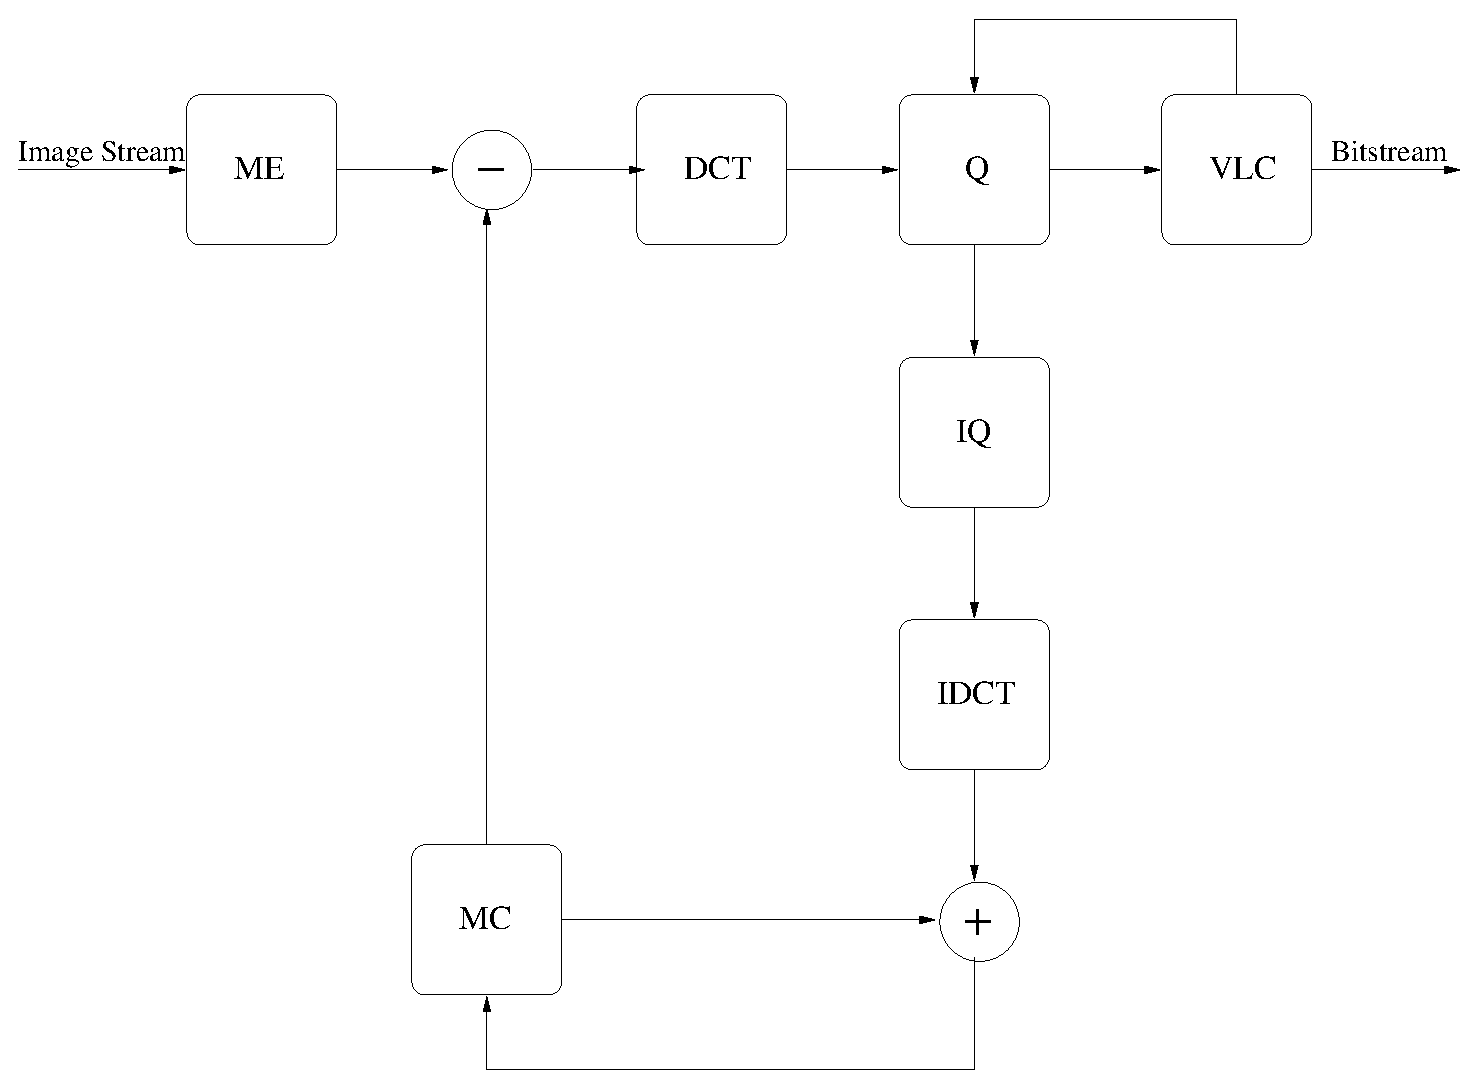
\epsfig{file=ec_block.eps,width=5in}}
\caption{Block diagram of MPEG-2 encode.}
\label{fig:ec_block}
\end{figure}

Our strategy for parallelizing MPEG-2 encoding is based on exploiting
data parallelism among slices.  Slices can be distributed across
streams, and each stream performs all operations independently, except
for motion estimation.

During motion estimation streams need to search through reference
frames to find the best match for the macroblock currently being
encoded.  At this point, inter-stream communication occurs as streams
send each other their locally stored slices of the reference frame.
This communication occurs every time a macroblock is predictively
coded.

The MPEG-2 standard does not specify a minimum or maximum search
window for motion estimation.  It could be as large as the entire
reference frame or as small as a few pixels.  In the case where the
encoder searches the entire reference frame, every stream has to
broadcast its reference slices to all other streams.  This all-to-all
communication can be very inefficient and generally does not scale
well for large numbers of streams.

We exploit the fact that the MPEG-2 standard does not specify a
maximum search window to implement a more efficient communication
scheme. Specifically, we impose a maximum length on motion vectors
produced by our encoder.  This upper bound on motion vector length
limits the potential number of reference macroblocks for a
predictively coded macroblock.  Such an implementation does not
broadcast reference data to all streams, but confines communication to
the sets of streams whose search windows overlap.  Furthermore, by
ensuring that adjacent ranges of macroblocks are allocated to adjacent
streams, this implementation can ensure that communication is local,
as illustrated in Figure~\ref{fig:mb_alloc}.  Such local communication
patterns allow this implementation to scale much more efficiently as
the number of streams grows.

The maximum search window size is a parameter which can be tuned on a
case by case basis.  Larger search windows have the potential for
finding better matches and thus a more compact encoding.  Smaller
search windows limit the amount of communication, offering faster
performance at the cost of either less compression or lower quality
images.  The ideal window size depends on the number of streams, the
size of the frames, and the relative importance of encoder speed and
output quality.

\begin{figure}[htbp]
\centerline{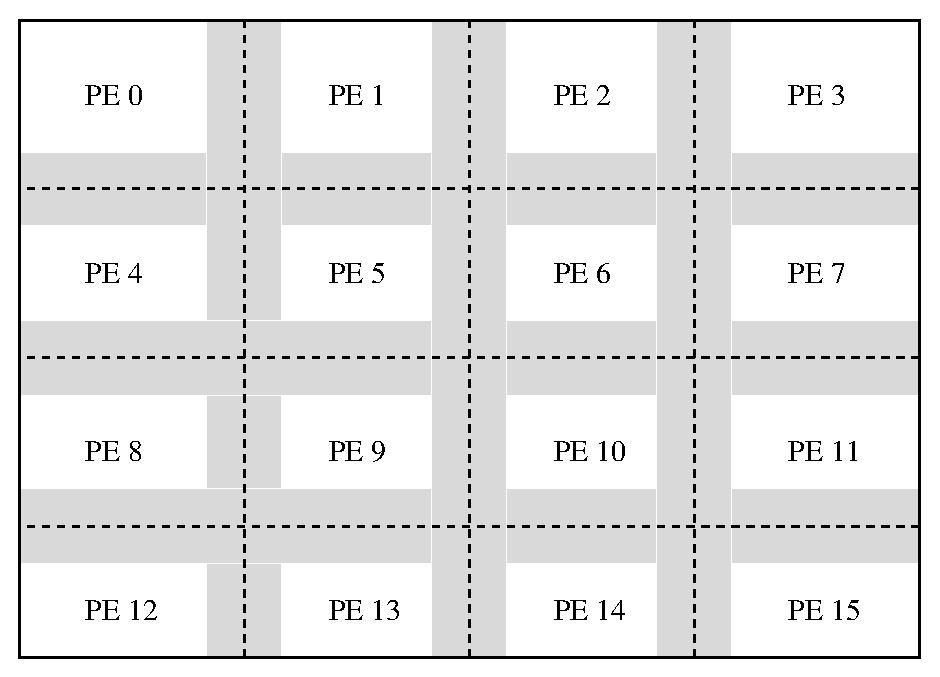
\epsfig{file=mb_alloc.eps,width=5in}}
\caption{Potential allocation of a reference frame among sixteen
streams.  Regions in gray represent reference macroblocks that are
communicated among neighboring streams.  The width of the gray
region represents the maximum motion vector size.}
\label{fig:mb_alloc}
\end{figure}

While using a fixed maximum search window can benefit performance by
reducing the amount of communication overhead, it can be quite
complicated to implement the local communication patterns on actual
hardware.  However, StreamIt provides mechanisms which allow
programmers to expose these local communication patterns to the
compiler.  The compiler handles the burden of allocating streams to
hardware resources and scheduling local communication. The remainder
of this section illustrates these concepts in the context of MPEG-2
encoding.

  \section{Related Work}
\label{sec:related}

Software pipelining for clustered vliws \cite{qian02}.

The Imagine stream processor~\cite{rixner98bandwidthefficient}
supports a time-multiplexed execution model.  The architecture
contains 48 parallel ALU's organized into 6 VLIW clusters.  The
programming model requires the programmer to write computation filters
in Kernel-C and stitch them together using Stream-C.  Because the
execution unit is data-parallel, the compiler uses time multiplexing
to execute a single filter at a time across all of the parallel
clusters.  While this provides perfect load balancing and high
arithmetic utilization when there is abundant data parallelism, it
suffers when a filter has retained state or data-dependences between
iterations.  Moreover, architectures based solely on
time-multiplexing do not scale spatially, as there are global wires
orchestrating the parallel execution units. 

Previous work in compiling StreamIt to Raw has taken a purely space
multiplexed approach~\cite{streamit-asplos}.  In this model, a single
filter was mapped to each execution tile.  To support applications
with more filters than execution tiles, a partitioning algorithm was
employed to adjust the granularity of the graph by fusing adjacent
filters into one.

Previous work in scheduling computation graphs to parallel targets
have focused on dynamic techniques \cite{SDFSched, SDFSched2,
may87communicating, DAGSched}. In general, multiple graph nodes are
{\it clustered} onto a single computational node and scheduled
dynamically.  

Our work, unlike most previous work in this field,
models link contention and topography.  Furthermore, StreamIt graphs
are implicitly formed of loops so we can apply loop scheduling
techniques such as software pipelining to build our schedules.

%The problem of instruction scheduling for MIMD and VLIW architectures
%is similar to the problem tackled by the space-time compiler.  ILP
%compilers for clustered VLIW architectures~\cite{Bulldog, Multiflow}
%are decomposed into stages that are analogous to the stages of the
%SpaceTime compiler.  These compilers must partition or cluster
%instructions, assign instructions to processors, and then schedule the
%instructions.  

Previous work on software pipelining has focused on scheduling machine
instructions in a loop \cite{lam-softpipe, rau-softpipe} to a
uniprocessor target.  The algorithms devised must account for tight
resource constraints and complex instruction dependences.  Our
software-pipelining problem is much less constrained, a traditional
modulo scheduling algorithm can not effectively take advantage of this
flexibility.  Previous work on ILP scheduling for the Raw
architectures ~\cite{lee98spacetime} also bears similarity.  However,
these compilers schedule graphs of fine-grained instructions. The
partitioning and scheduling heuristics are mindful of a different set
of constraints including different types of dynamism and less regular
communication patterns as compared to StreamIt graphs.

As far as we know, we are the first to apply loop-level scheduling
techniques to the problem of scheduling coarse-grained task graphs.

% \cite{cheops-thesis}
%   http://web.media.mit.edu/~kung/publication/thesis.pdf
%
% other possible things to cite:
%  http://portal.acm.org/citation.cfm?id=801721&dl=ACM&coll=portal
%  http://www.csrl.unt.edu/~kavi/Research/ica3pp156.pdf
%  http://cdmetcalf.home.comcast.net/papers/cop/node1.html#SECTION00010000000000000000

  %\section{Future Work}
\label{sec:future}

%% First, as the current transformation has the potential to increase the
%% size of the file, we plan to explore lightweight techniques for
%% re-compressing a data stream that is already partially compressed.
%% This should be straightforward in the case of Apple Animation; for
%% example, a run-length encoded unit can be extended without needing to
%% be rediscovered.

There remain rich areas for future work in computing on compressed
data.  First, the compressed processing technique can be applied far
beyond the current focus.  In its current form, the technique could be
evaluated on video operations such as thresholding, color depth
reduction, sepia toning, saturation adjustment, and color replacement.
With minor extensions (see Section~\ref{sec:extensions}), the
technique can support video operations such as cropping, padding,
histograms, image flipping, sharpening, and blurring.  The technique
may also have applications in an embedded setting, where it could
offer power savings---for example, in processing the RAW data format
within digital cameras.  It may even be possible to do sparse matrix
operations using the technique; in addition to compressing the
locations of the zero elements, LZ77 would also compress repetetive
patterns in the non-zero elements.

Research is also underway to apply a similar technique to lossy,
DCT-based compression formats.  The streaming model cf computation
also offers key advantages in this domain, as neighboring actors that
compute linear functions can be algebraically simplified at compile
time~\cite{aalamb}.  For example, a JPEG transcoder typically performs
an iDCT (during decompression), followed by the user's transformation,
followed by a DCT (during compression).  If the user's transformation
is also linear (e.g., color inversion) then all three stages can be
automatically collapsed, thereby eliminating the decompression and
re-compression steps.  Preliminary experiments in this direction
indicate speedups upwards 10x.  By extending the framework to multiple
compression formats, users will be able to write their transformations
once, in a high-level language, and rely on the compiler to map the
computations to each of the compresed domains.


  \section{Conclusions and Future Work}
\label{sec:conclusion}

This paper makes two contributions.  First, it introduces teleport
messaging: a powerful language construct enabling precise message
delivery between nodes of a distributed stream program.  In comparison
with other methods to implement messaging functionality in a
Synchronous Dataflow (SDF) model, teleport messaging is arguably more
readable, more robust, and easier to maintain.  In addition, our
implementation of teleport messaging in the StreamIt compiler resulted
in a 49\% performance improvement for a frequency hopping radio
running on a cluster of workstations.  Like several declarative
language constructs, teleport messaging improves performance by
exposing the true dependences to the compiler and allowing it to
optimize the communication.

%% We outlined several possible applications of $\sdep$, including
%% latency constraints, debugging, speculation, and program analysis, and
%% we look forward to pursuing these directions in the future.

Second, this paper formulates $\sdep$, a natural and useful dependence
representation for the streaming domain.  While this paper applies
$\sdep$ to a new language construct, we envision other applications as
well.  For example, $\sdep$ could be used in a debugger to identify
which iterations of an upstream actor are affecting a given iteration
of a downstream actor.  In a software-based speculation
system~\cite{frank-thesis}, $\sdep$ could be applied to trace the
effects of a failed prediction and to roll back the appropriate actor
executions.  $\sdep$ also offers a new method for measuring latency in
a stream graph.  Similar to representations such as dependence
levels~~\cite{AK82}, direction vectors~\cite{wolfe82}, and dependence
polyhedra~\cite{Irig88} for scientific programs, $\sdep$ provides
dependence information that could be used to test or verify program
transformations.

There are some limitations in the current study that are fertile
grounds for future research.  First, our formulation of $\sdep$
requires a directed path in the stream graph (aligned with the
direction of data flow) between the actors in question.  We are
generalizing $\sdep$ to actors that run in parallel by leveraging
their data dependences with common predecessors (upstream) or
successors (downstream).  Second, as detailed in
Section~\ref{sec:constraints}, we do not solve the general scheduling
problem that incorporates overlapping constraints from teleport
messaging; even determining whether or not a set of constraints is
feasible (especially during the initialization
schedule~\cite{karczma-thesis}) seems to be an interesting question.
Third, in the current model only actors can send and receive messages.
We are extending this into a hierarchical model where stream
containers (such as pipelines) can also receive events and dispatch
them precisely to other streams.  Finally, our approach relies on the
static communication rates present in SDF.  It would be interesting to
consider teleport messaging in a more dynamic context; for example,
downstream non-negative latency messages could be immediately
supported by embedding messages in data items, while other messages
might require speculative delivery or modified timing contracts.

Our work can be viewed as the integration of dynamic behavior into a
static dataflow language.  Our insight is that there is a class of
control messages that only adjust a parameter in the target actor;
they do not otherwise affect the input or output channels upon
delivery.  This model enables a hybrid scheduling scheme in which the
steady-state dataflow is exactly orchestrated at compile time, but
there are windows in which a message could adjust an internal field of
an actor between its execution steps.  We consider this to be a
promising avenue for creating a unified development environment that
captures all aspects of stream application development without
sacrificing either performance or programmability.

  
  \vspace{-2pt}
  \section*{Acknowledgements}
  \vspace{-7pt}
  We are very grateful to the entire StreamIt team for their hard work
  and insightful comments. Allyn Dimock, Michael Gordon, Janis
  Sermulins, and especially William Thies, contributed immensely to
  the StreamIt infrastructure to enable this paper. We also thank the
  anonymous reviewers for their helpful suggestions. The StreamIt
  project is supported by DARPA grants PCA-F29601-03-2-0065 and
  HPCA/PERCS-W0133890, and NSF awards CNS-0305453 and EIA-0071841.

%  \bibliographystyle{ipdps}
%  \bibliography{main}
  \vspace{-2pt}
\begin{thebibliography}{10}\setlength{\itemsep}{-1ex}\small
  \vspace{-7pt}
\bibitem{agrawal05cases}
S.~Agrawal, W.~Thies, and S.~Amarasinghe.
\newblock Optimizing stream programs using linear state space analysis.
\newblock In {\em {CASES}}, 2005.

\bibitem{ahmad01multiproc}
I.~Ahmad, S.~M. Akramullah, M.~L. Liou, and M.~Kafeel.
\newblock {A Scalable Off-line MPEG-2 Video Encoding Scheme using a
  Multiprocessor System}.
\newblock {\em {Parallel Computing}}, 27, 2001.

\bibitem{ahmad01compression}
I.~Ahmad, Y.~He, and M.~L. Liou.
\newblock {Video compression with parallel processing}.
\newblock {\em {Parallel Computing}}, 28, 2002.

\bibitem{ph}
S.~Aidtya, Arvind, L.~Augustsson, J.~Maessen, and R.~S. Nikhil.
\newblock {Semantics of pH: A parallel dialect of Haskell}.
\newblock In {\em Haskell Workshop}, 1995.

\bibitem{Lucid77}
E.~Ashcroft and W.~Wadge.
\newblock Lucid, a non procedural language with iteration.
\newblock {\em C. ACM}, 20(7), 1977.

\bibitem{assayad05mpeg4b}
I.~Assayad, P.~Gerner, S.~Yovine, and V.~Bertin.
\newblock {Modelling, Analysis and Parallel Implementation of an On-line Video
  Encoder}.
\newblock In {\em {1st Int. Conf. on Distributed Frameworks for Multimedia
  Applications}}, 2005.

\bibitem{Esterel}
G.~Berry and G.~Gonthier.
\newblock {The Esterel Synchronous Programming Language: Design, Semantics,
  Implementation}.
\newblock {\em Sci. of Comp. Programming}, 19(2), 1992.

\bibitem{brook04}
I.~Buck, T.~Foley, D.~Horn, J.~Sugerman, K.~Fatahalian, M.~Houston, and
  P.~Hanrahan.
\newblock {Brook for GPUs: Stream Computing on Graphics Hardware}.
\newblock In {\em SIGGRAPH}, 2004.

\bibitem{Lucid-Synchrone}
P.~Caspi and M.~Pouzet.
\newblock {Lucid Synchrone distribution}.
\newblock {\tt http://www-spi.lip6.fr/lucid-synchrone/}.

\bibitem{spidle03}
C.~Consel, H.~Hamdi, L.~R�veill�re, L.~Singaravelu, H.~Yu, and C.~Pu.
\newblock {Spidle: A DSL Approach to Specifying Streaming Application}.
\newblock In {\em {2nd Int. Conf. on Generative Prog. and Component
  Engineering}}, 2003.

\bibitem{Occam}
I.~Corporation.
\newblock {\em Occam 2 Reference Manual}.
\newblock Prentice Hall, 1988.

\bibitem{kock02jpeg}
E.~de~Kock.
\newblock {Multiprocessor Mapping of Process Networks: A JPEG Decoding Case
  Study}.
\newblock In {\em {15th Int. Symp. on System Synthesis}}, 2002.

\bibitem{kock00yapi}
E.~de~Kock, G.~Essink, W.~Smits, P.~van~der Wolf, J.~Brunel, W.~Kruijtzer,
  P.~Lieverse, and K.~Vissers.
\newblock {YAPI: Application Modeling for Signal Processing Systems}.
\newblock In {\em {Conf. on Design Automation}}, 2000.

\bibitem{dwivedi01exploring}
B.~K. Dwivedi, J.~Hoogerbrugge, P.~Stravers, and M.~Balakrishnan.
\newblock {Exploring design space of parallel realizations: MPEG-2 decoder case
  study}.
\newblock In {\em {9th Int. Symp. on Hardware/Software Codesign}}, 2001.

\bibitem{sisal}
J.~Gaudiot, W.~Bohm, T.~DeBoni, J.~Feo, and P.~Mille.
\newblock {The Sisal Model of Functional Programming and its Implementation}.
\newblock In {\em {2nd Aizu Int. Symposium on Parallel Algorithms/Architecture
  Synthesis}}, {1997}.

\bibitem{Signal}
T.~Gautier, P.~L. Guernic, and L.~Besnard.
\newblock Signal: A declarative language for synchronous programming of
  real-time systems.
\newblock {\em Springer Verlag LNCS}, 274, 1987.

\bibitem{gordon02asplos}
M.~Gordon, W.~Thies, M.~Karczmarek, J.~Lin, A.~S. Meli, C.~Leger, A.~A. Lamb,
  J.~Wong, H.~Hoffman, D.~Z. Maze, and S.~Amarasinghe.
\newblock {A Stream Compiler for Communication-Exposed Architectures}.
\newblock In {\em {ASPLOS}}, 2002.

\bibitem{Lustre}
N.~Halbwachs, P.~Caspi, P.~Raymond, and D.~Pilaud.
\newblock The synchronous data flow language {LUSTRE}.
\newblock {\em Proc. of the IEEE}, 79(1), 1991.

\bibitem{MPEG2}
{ISO/IEC 11172: Information technology --- Coding of moving pictures and
  associated audio for digital storage media at up to about 1.5 Mbit/s}.
\newblock {International Organization for Standardization}, 1999.

\bibitem{iwata98coarse}
E.~Iwata and K.~Olukotun.
\newblock {Exploiting coarse-grain parallelism in the MPEG-2 algorithm}.
\newblock Technical Report {CSL-TR-98-771}, Stanford University, 1998.

\bibitem{imagine03ieee}
U.~J. Kapasi, S.~Rixner, W.~J. Dally, B.~Khailany, J.~H. Ahn, P.~Mattson, and
  J.~D. Owens.
\newblock Programmable stream processors.
\newblock {\em IEEE Computer}, 2003.

\bibitem{ko05dgt}
D.-I. Ko and S.~S. Bhattacharyya.
\newblock {Dynamic Configuration of Dataflow Graph Topology for DSP System
  Design}.
\newblock In {\em {ICASSP}}, 2005.

\bibitem{bhatta05block}
D.-I. Ko and S.~S. Bhattacharyya.
\newblock {Modeling of Block-Based DSP Systems}.
\newblock {\em {Journal of VLSI Signal Processing}}, 40(3), 2005.

\bibitem{cossap}
J.~Kunkel.
\newblock {COSSAP: A stream driven simulator}.
\newblock In {\em {Int. Workshop on Microelectronics in Communications}}, 1991.

\bibitem{lamb03pldi}
A.~A. Lamb, W.~Thies, and S.~Amarasinghe.
\newblock {Linear Analysis and Optimization of Stream Programs}.
\newblock In {\em {PLDI}}, 2003.

\bibitem{grape-ii}
R.~Lauwereins, M.~Engels, M.~Ad\'e, and J.~Peperstraete.
\newblock {Grape-II: A System-Level Prototyping Environment for DSP
  Applications}.
\newblock {\em {IEEE Computer}}, 28(2), 1995.

\bibitem{lee87static}
E.~Lee and D.~Messershmitt.
\newblock {Static Scheduling of Synchronous Data Flow Programs for Digital
  Signal Processing}.
\newblock {\em IEEE Trans. on Computers}, C-36(1), 1987.

\bibitem{ptolemy03overview}
E.~A. Lee.
\newblock {Overview of the Ptolemy Project}.
\newblock Technical report, UCB/ERL M03/25, UC Berkeley, 2003.

\bibitem{li05alpbench}
M.-L. Li, R.~Sasanka, S.~V. Adve, Y.-K. Chen, and E.~Debes.
\newblock {The ALPBench Benchmark Suite for Complex Multimedia Applications}.
\newblock In {\em {IEEE Int. Symp. on Workload Characterization}}, 2005.

\bibitem{cg03}
W.~R. Mark, R.~S. Glanville, K.~Akeley, and M.~J. Kilgard.
\newblock {Cg: A System for Programming Graphics Hardware in a C-like
  Language}.
\newblock In {\em SIGGRAPH}, 2003.

\bibitem{yelick04msp}
M.~Narayanan and K.~A. Yelick.
\newblock Generating permutation instructions from a high-level description.
\newblock In {\em Workshop on Media and Streaming Processors}, 2004.

\bibitem{neuendorffer04hierarchical}
S.~Neuendorffer and E.~Lee.
\newblock {Hierarchical Reconfiguration of Dataflow Models}.
\newblock In {\em {Conference on Formal Methods and Models for Codesign}},
  2004.

\bibitem{park99spdf2}
C.~Park, J.~Chung, and S.~Ha.
\newblock {Efficient Dataflow Representation of MPEG-1 Audio (Layer III)
  Decoder Algorithm with Controlled Global States}.
\newblock In {\em {IEEE Workshop on Signal Processing Systems}}, 1999.

\bibitem{park02spdf3}
C.~Park, J.~Jung, and S.~Ha.
\newblock {Extended Synchronous Dataflow for Efficient DSP System Prototyping}.
\newblock {\em {Design Automation for Embedded Systems}}, 6(3), 2002.

\bibitem{pazos04soc}
N.~Pazos, P.~Ienne, Y.~Leblebici, and A.~Maxiaguine.
\newblock {Parallel Modelling Paradigm in Multimedia Applications: Mapping and
  Scheduling onto a Multi-Processor System-on-Chip Platform}.
\newblock In {\em {Int. Global Signal Processing Conference}}, 2004.

\bibitem{pelayo01rosa}
F.~L. Pelayo, F.~Cuartero, V.~Valero, D.~Cazorla, and T.~Olivares.
\newblock {Specification and Performance of the MPEG-2 Video Encoder by Using
  the Stochastic Process Algebra: ROSA}.
\newblock In {\em {17th UK Performance Evaluation Workshop}}, 2001.

\bibitem{sermulins05lctes}
J.~Sermulins, W.~Thies, R.~Rabbah, and S.~Amarasinghe.
\newblock {Cache Aware Optimization of Stream Programs}.
\newblock In {\em {LCTES}}, 2005.

\bibitem{shen94overview}
K.~Shen, G.~Cook, L.~Jamieson, and E.~Delp.
\newblock {Overview of parallel processing approaches to image and video
  compression}.
\newblock In {\em {SPIE Conference on Image and Video Compression}}, 1994.

\bibitem{survey97}
R.~Stephens.
\newblock {A Survey of Stream Processing}.
\newblock {\em Acta Informatica}, 34(7), 1997.

\bibitem{streamitcc}
W.~Thies, M.~Karczmarek, and S.~Amarasinghe.
\newblock {StreamIt: A Language for Streaming Applications}.
\newblock In {\em {Int. Conf. on Compiler Construction}}, {2002}.

\bibitem{thies05ppopp}
W.~Thies, M.~Karczmarek, J.~Sermulins, R.~Rabbah, and S.~Amarasinghe.
\newblock Teleport messaging for distributed stream programs.
\newblock In {\em PPoPP}, 2005.

\bibitem{valero02petri}
V.~Valero, F.~L. Pelayo, F.~Cuartero, and D.~Cazorla.
\newblock {Specification and Analysis of the MPEG-2 Video Encoder with
  Timed-Arc Petri Nets}.
\newblock {\em {Electronic Notes in Theoretical Computer Science}}, 66(2),
  2002.

\bibitem{reference-mpeg-c}
{VMPEG (Reference C Code). ftp://ftp.mpegtv}.
\newblock com/pub/mpeg/mssg/mpeg2vidcodec\_v12.tar.gz.

\end{thebibliography}

\end{document}
